The purpose of this test is to test the observer based LQR (OBLQR) controller on the Hi-Fi simulation. Focus will be on how the cargo hold air temperature and evaporator output refrigerant temperature reacts, when the model is near the operating point and when different disturbances are applied. Additionally, the power consumption for the actuators of the observer based controller will be compared to the power consumption for the actuators of the PID controller.

\subsection{Test framework}
When the HiFi simulation model is initialized, the system takes approximately 1.5 hours until it converges to steady state. Since the OBLQR controller is not expected to work well when operating far from the linearisation point, the existing PID control structure is used to handle the initial transient behavior. This is done as not all of the states in the Hi-Fi simulation model are available. Thus, they can not be initialised at the operating point, and in stead the PID controller is used to bring the system \textbf{near} the operating point before the OBLQR controller can be applied. 
As the simulation model is deterministic, it is possible to choose a fixed time when the OBLQR controller can take over, and then know that the system is some fixed distance from the operating point. This is used to show whether the OBLQR controller can handle deviations from the operating point.

\begin{figure}[h!]
	\centering
	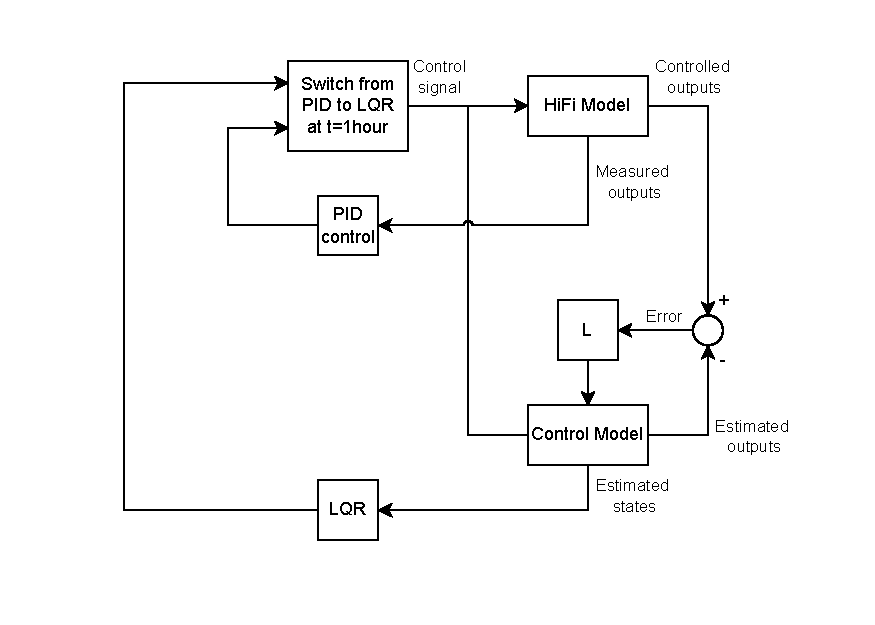
\includegraphics[width=0.8\textwidth]{Graphics/HiFi_simulation_test_diagram.pdf}
	\caption{Top: Cargo hold air temperature. $T_0$ = -4.25$^{\circ}$C. Bottom: Evaporator vapor refrigerant temperature. $T_0$ = -5.55$^{\circ}$C}
	\label{fig:test_setup}
\end{figure}

The test setup is sketched in \cref{fig:test_setup}. A switch is inserted in the simulation which changes the inputs to the Hi-Fi simulation from the PID control structure to the LQR controller at some specified time. It takes two inputs: the vector of the PID chosen control inputs and the vector of the OBLQR controller input. The PID control structure inputs are fed to the system until the time reaches 1 hour, at which point the states will be \textbf{near} the linearisation point. At this point, the switch selects the OBLQR control inputs to be fed to the system. Until the switching time, the control model (observer) states are forced to stay at 0.

Two simulations will run in parallel: The above described, and one where the PID control structure continues to regulate the system for the entire simulation. This allows for comparison between the two control strategies.\\

Three scenarios are simulated:

\begin{enumerate}
	\item No disturbance (at operating point)
	\item Sine wave disturbance
	\item Step away from operating point disturbance
\end{enumerate}

\noindent For each of the three scenarios the two outputs, namely the cargo hold air temperature and evaporator output refrigerant temperature are plotted along with the controller inputs. The two outputs are plotted from both the Hi-Fi simulation and the observer to see whether the observer successfully estimates those two states. Furthermore the output of the Hi-Fi model is plotted when its own PID controller structure inputs are fed to it to benchmark it against the LQR controller. Lastly the average power consumption by the two control strategies are mentioned to evaluate the efficiency of the OBLQR.

\subsection{Tuned LQR controller: Constant disturbance}
This test illustrates the performance of the OBLQR controller in the best case scenario, namely where the disturbance (ambient temperature) is held constant at 20$^{\circ}$C. This is the operating point for the disturbance. The controlled outputs are seen in \cref{fig:LQR_wellTuned_noDist}. The OBLQR controller is set to start regulating the system at time $t=1$ hours, at which point it will attempt to drive the states to 0. This is done to illustrate whether the OBLQR controller can drive the states to zero when from outside the operating point.

\begin{figure}[H]
	\centering
	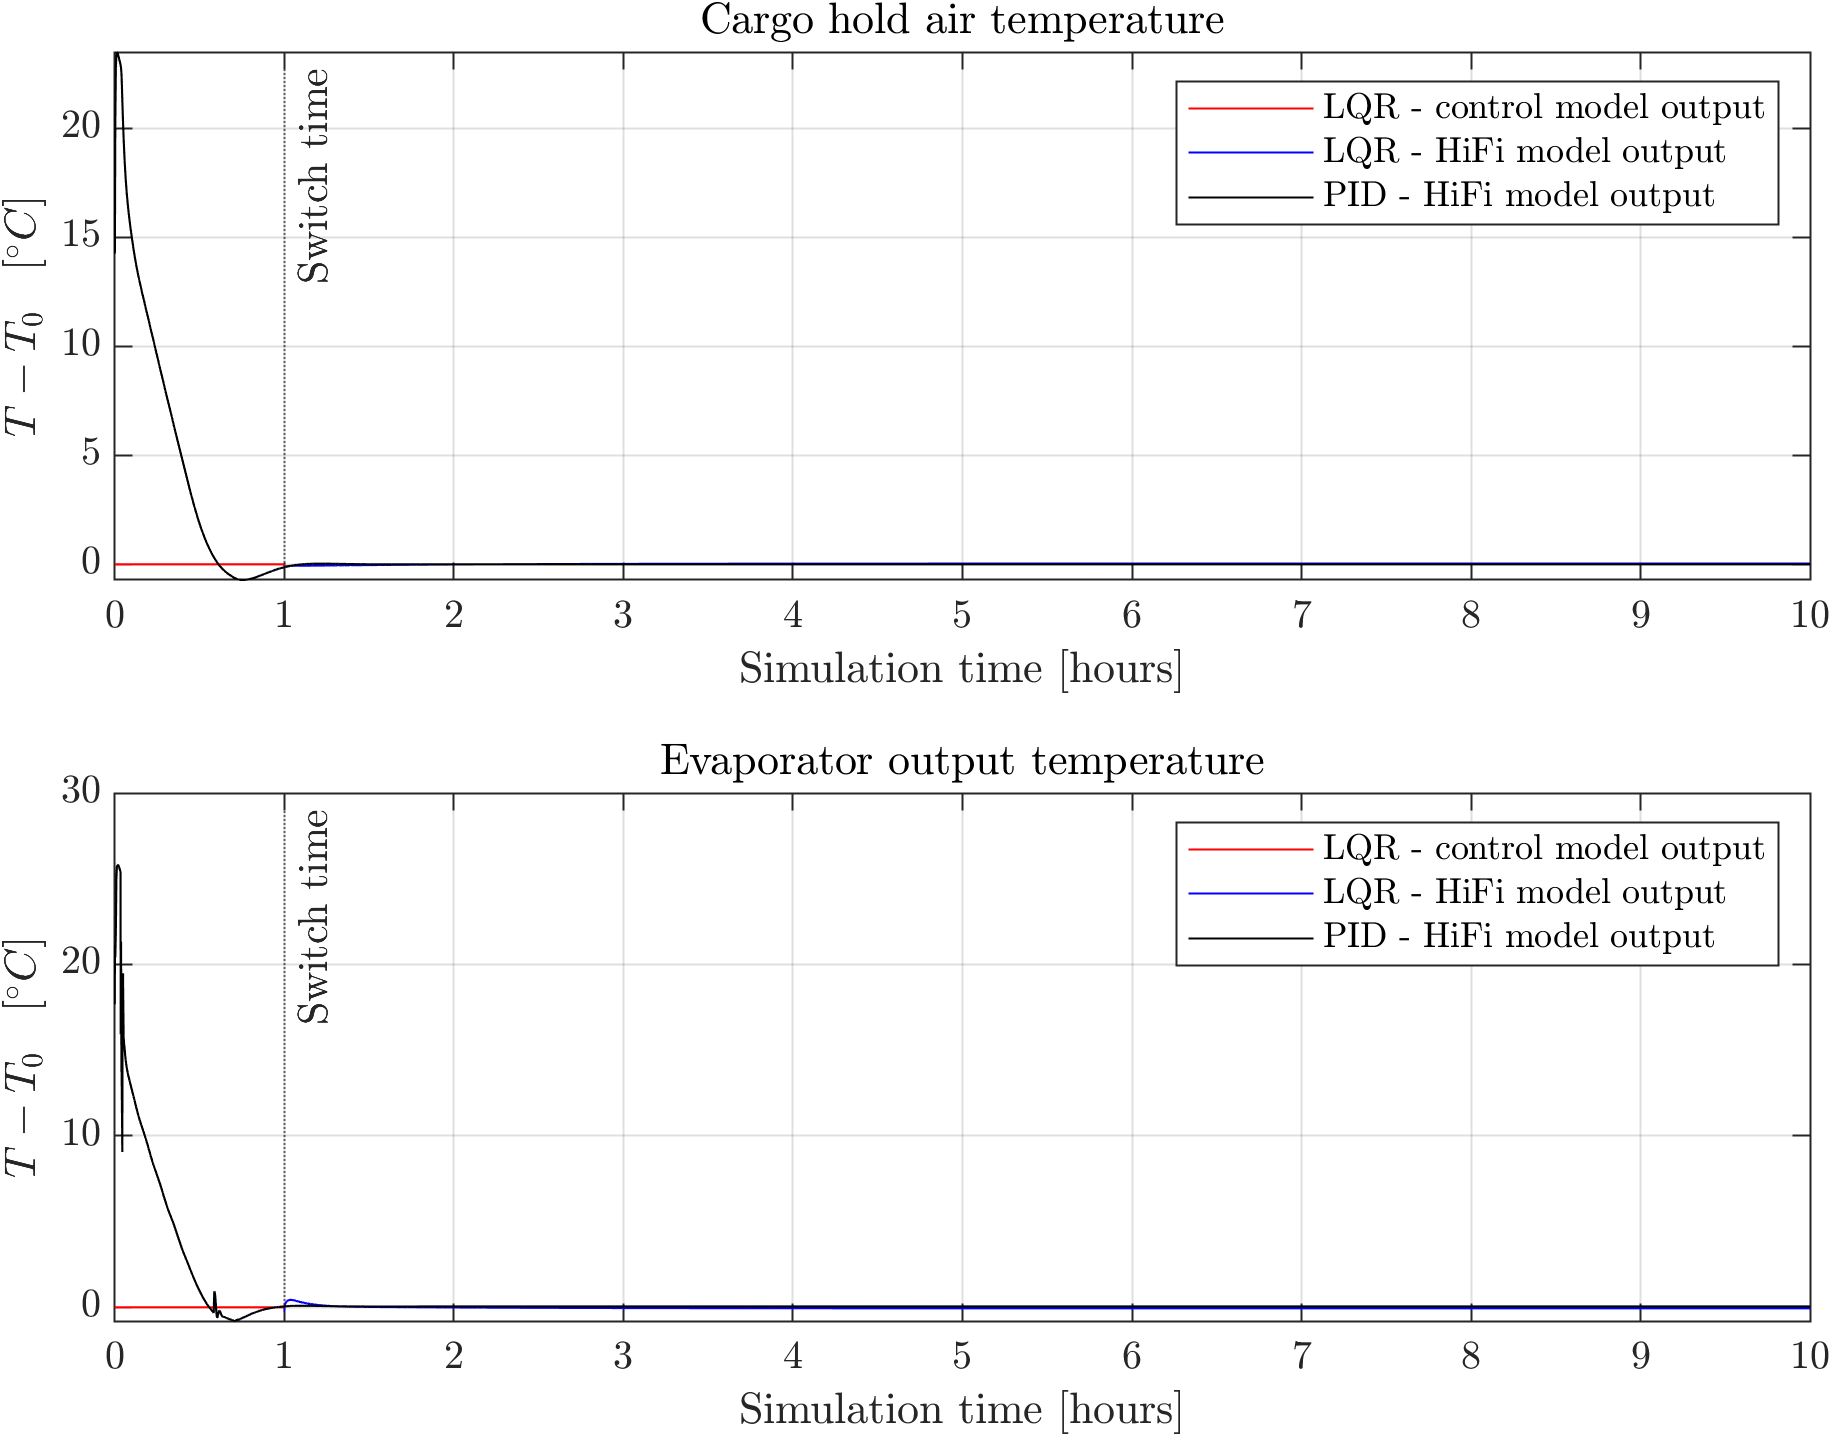
\includegraphics[width=0.8\textwidth]{Graphics/fig_LQRvsKresten_noDist.png}
	\caption{No disturbance case: Top: Cargo hold air temperature. $T_0$ = -4.25$^{\circ}$C. Bottom: Evaporator vapor refridgerant temperature. $T_0$ = -5.55$^{\circ}$C. The controlled outputs from both controllers are regulated near zero}
	\label{fig:LQR_wellTuned_noDist}
\end{figure} \todo[inline]{Remove observer estimated outputs for all figures. We need to focus on the actual outputs}
The controlled outputs of the OBLQR controller is regulated to near zero, and as such, the controller seem to work near the linearisation point. To further investigate the accuracy of the controlled outputs, a zoomed version of \cref{fig:LQR_wellTuned_noDist} is consulted in \cref{fig:LQR_wellTuned_noDist_zoom}.


\begin{figure}[H]
	\centering
	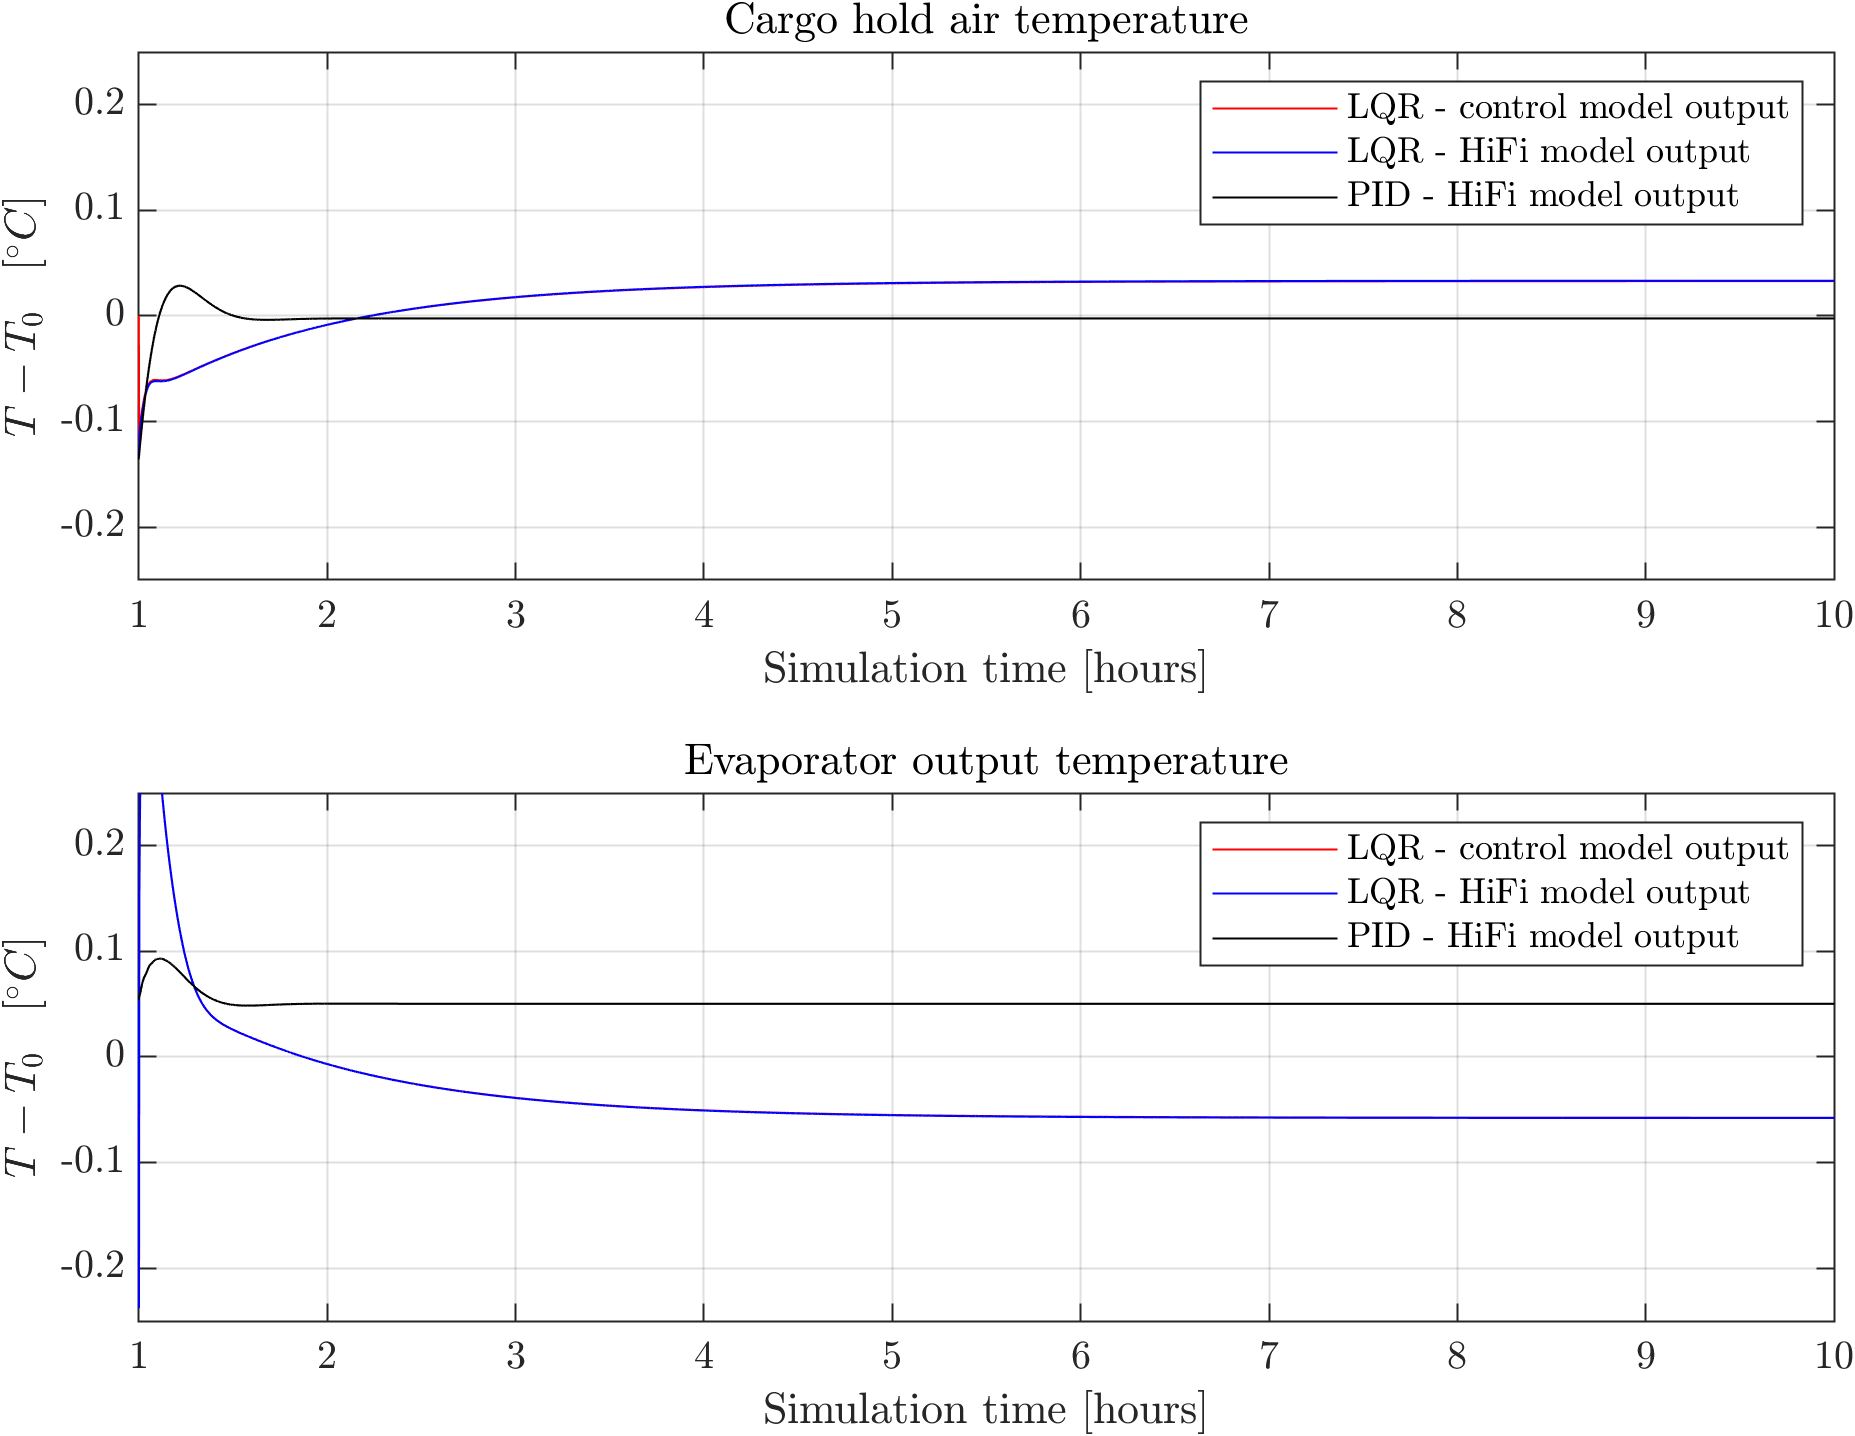
\includegraphics[width=0.8\textwidth]{Graphics/fig_LQRvsKresten_noDist_zoom.png}
	\caption{Zoomed version of \cref{fig:LQR_wellTuned_noDist}. No disturbance case: Top: Cargo hold air temperature. $T_0$ = -4.25$^{\circ}$C. Bottom: Evaporator vapor refridgerant temperature. $T_0$ = -5.55$^{\circ}$C. The OBLQR has a slight steady state error of about 0.03 $^{\circ}$C in the first subplot. In the second subplot it is -0.06 $^{\circ}$C. The settling time is longer for both cases than that of the PID controller}
	\label{fig:LQR_wellTuned_noDist_zoom}
\end{figure}

\noindent The error is so numerically small (0.02$^{\circ}$C for cargo temperature and 0.06 $^{\circ}$C evaporator output refrigerant temperature) that most real temperature sensors would be unable to detect it. The LQR controller is thus shown to be able to drive the system to practically zero, when no disturbance is present. The settling time is however noticeably longer than that of the PID controlled system. 

The control inputs during this test is seen in \cref{fig:inputs_noDist}. As expected the removed inputs are constant at the operating point, but perhaps less expected the remaining inputs $\Theta_1$ and $U_{fan2}$ do not change despite the air and evaporator output error.

\begin{figure}[H]
	\centering
	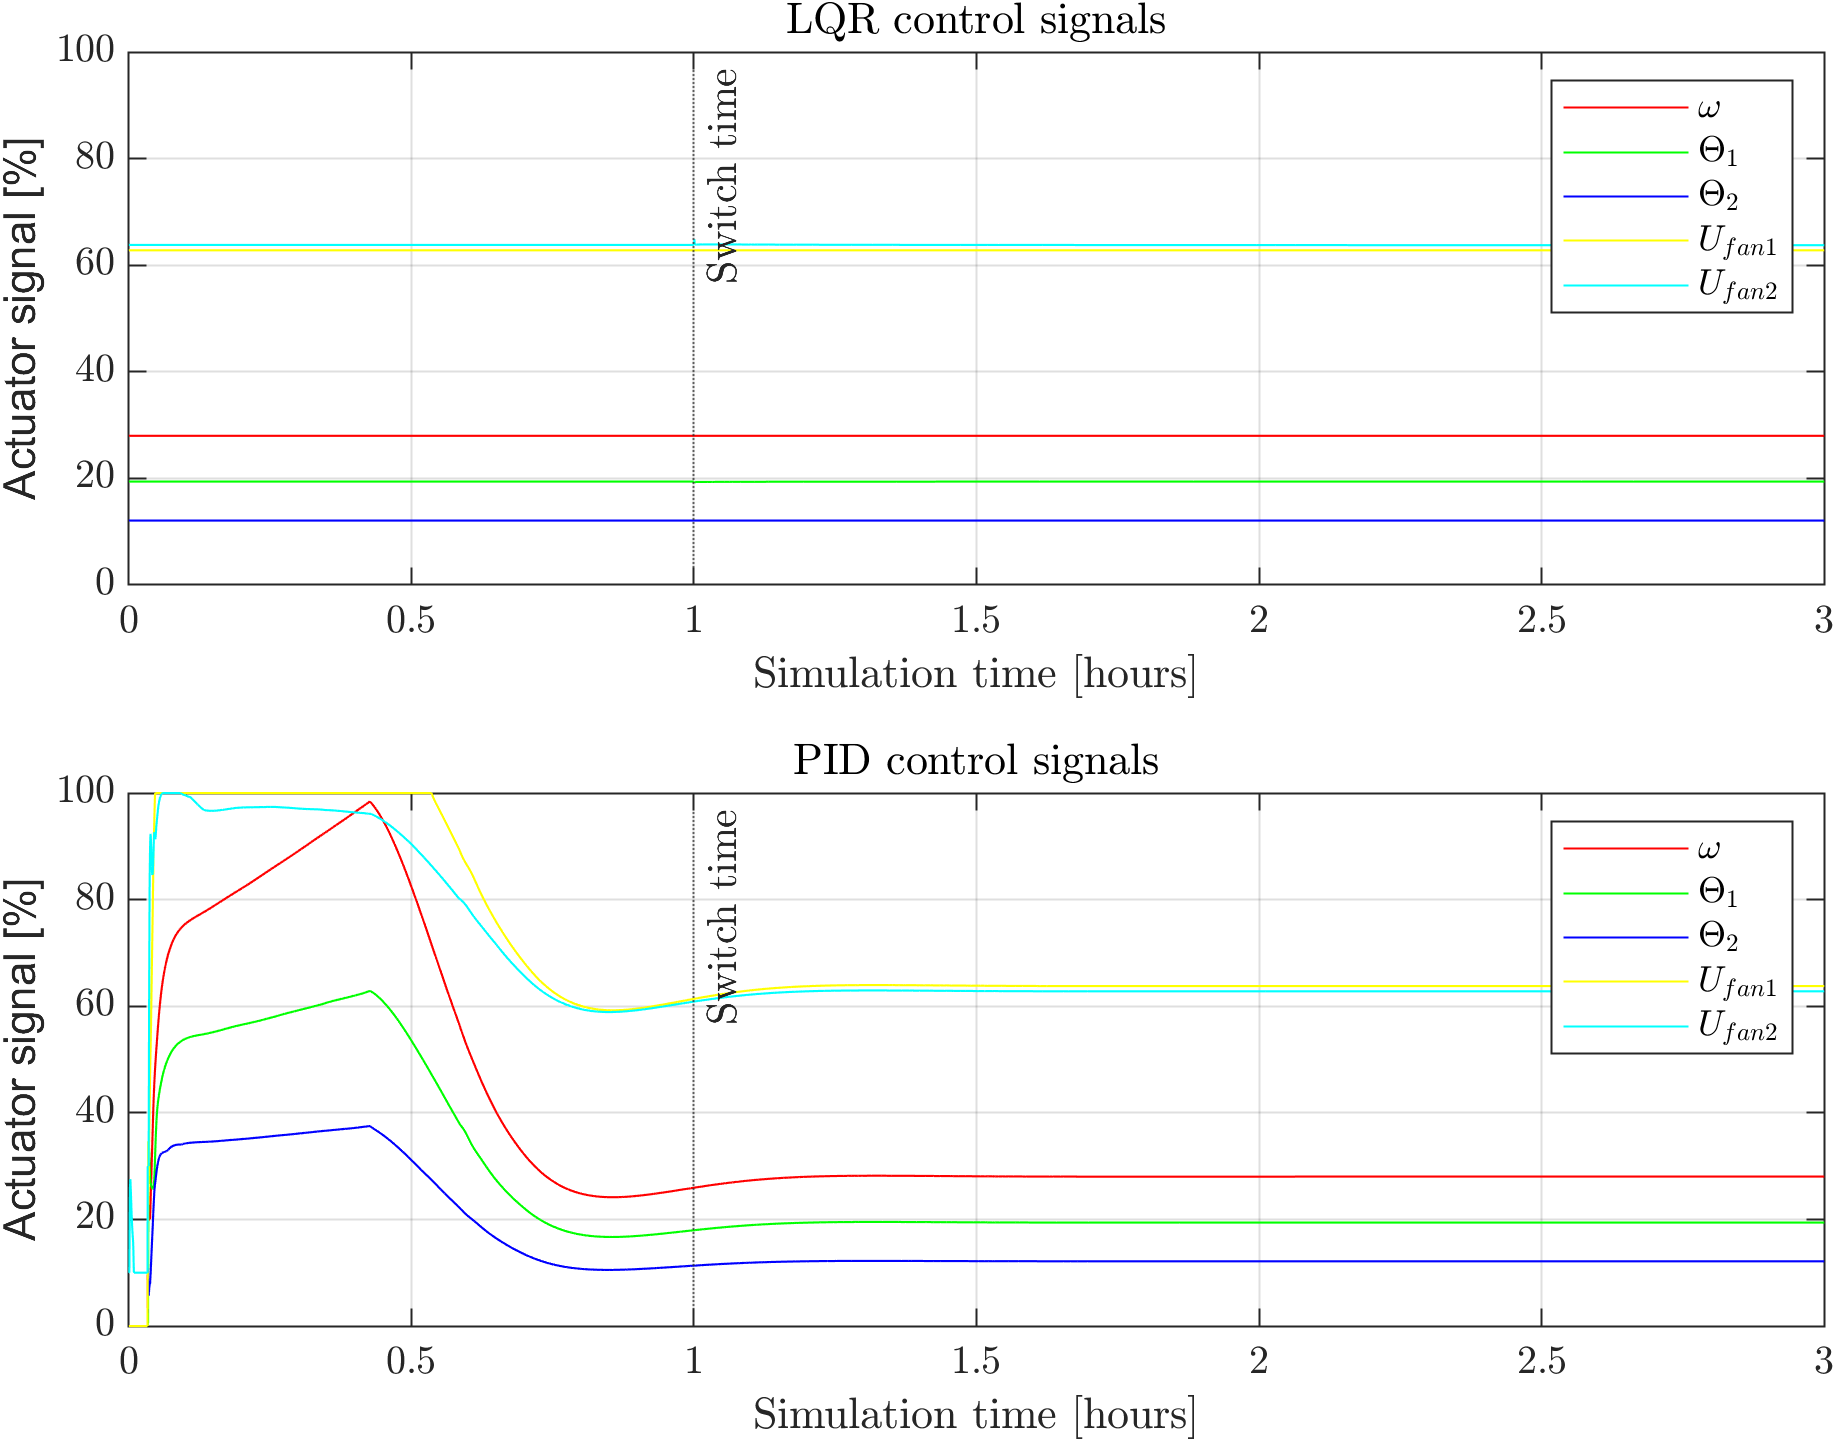
\includegraphics[width=0.8\textwidth]{Graphics/fig_inputs_noDist.png}
	\caption{No disturbance case: Plot of the control signals applied to the Hi-Fi Simulation. Top: LQR control signals. Bottom: Hi-Fi simulation PID control signals.}
	\label{fig:inputs_noDist}
\end{figure}
The fact that the OBLQR control signals $ \Theta_1, U_{fan2} $ seem to be constant is a bit surprising. It is therefore investigated closer by a zoomed plot in \cref{fig:inputs_noDist_zoom}.

\begin{figure}[H]
	\centering
	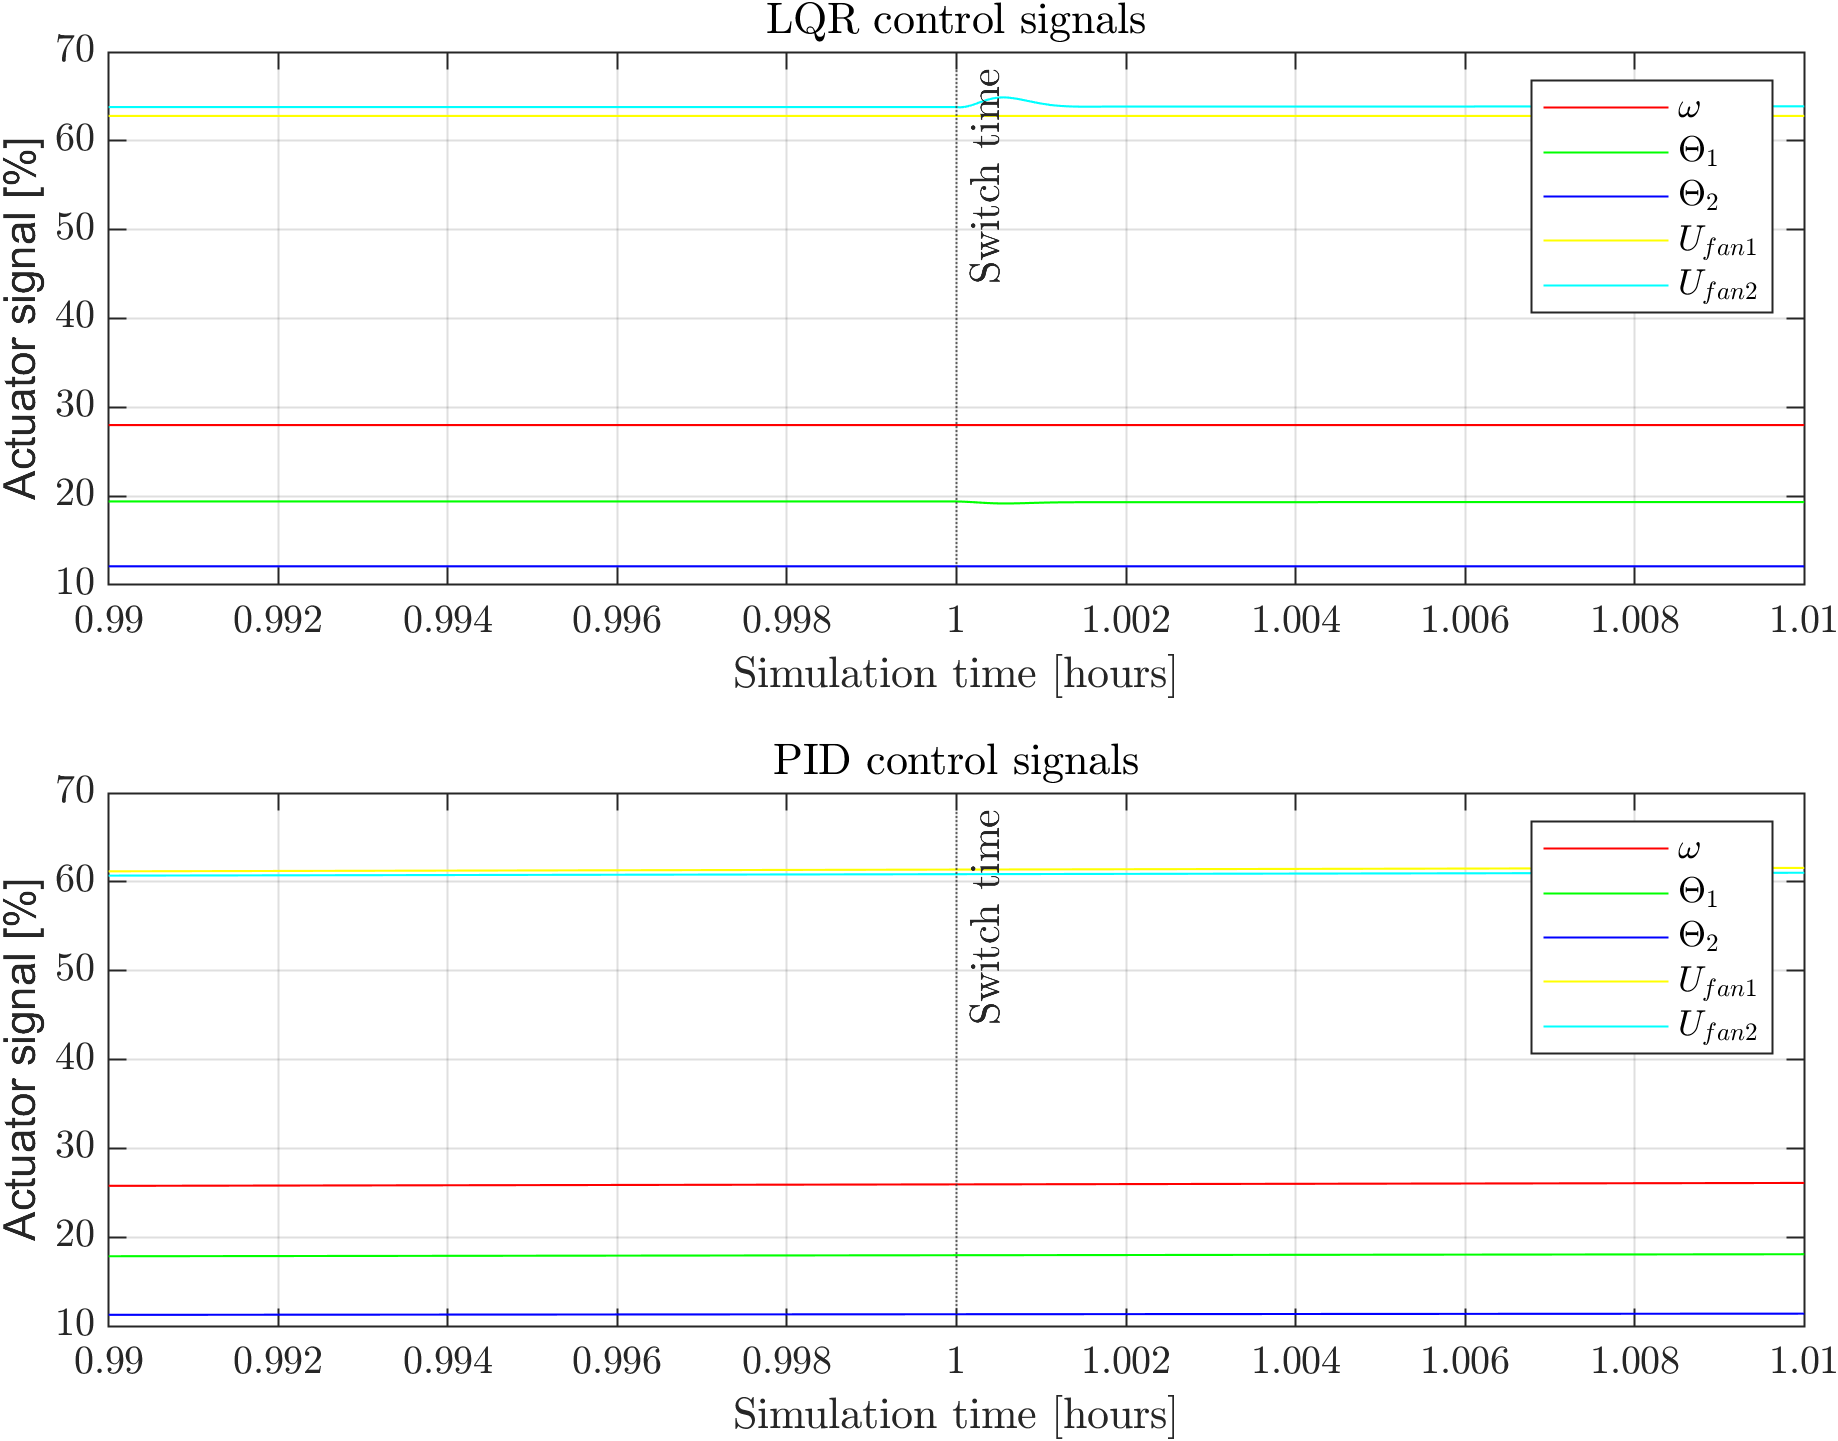
\includegraphics[width=0.8\textwidth]{Graphics/fig_inputs_noDist_zoom.png}
	\caption{Zoomed version of \cref{fig:inputs_noDist}. No disturbance case: Plot of the control signals applied to the Hi-Fi Simulation (zoomed). Top: LQR control signals. Bottom: Hi-Fi simulation PID control signals.}
	\label{fig:inputs_noDist_zoom}
\end{figure}
 
In \cref{fig:inputs_noDist_zoom}, it can be seen that $ \Theta_1, U_{fan2} $ are in fact varying slightly to, just after the switch time. This confirms that the controller is reacting to the controlled outputs. \\
\noindent As the linearised model of the OBLQR model is based on the same linearisation point as the steady state PID controllers, the power consumptions are very similiar. The power consumption in steady state for the two controllers are the same, XX W.

OBLQR: 25.22 kWh
PID: 25.14 kWh

\todo[inline]{Mention power consumption}

\newpage
\subsection{Tuned LQR controller: Sine disturbance}
The controllers dynamic performance is now investigated as a sine disturbance is applied to the system. As before, PID controller will handle the initial hour of settling. The LQR then starts regulating the system, and at time $t=3$ hours, the disturbance is injected to the ambient temperature. The disturbance is a sine wave with an amplitude of 5$^{\circ}$C and a period of 10 minutes. The controlled outputs are seen in \cref{fig:LQR_wellTuned_sineDist}.

\begin{figure}[H]
	\centering
	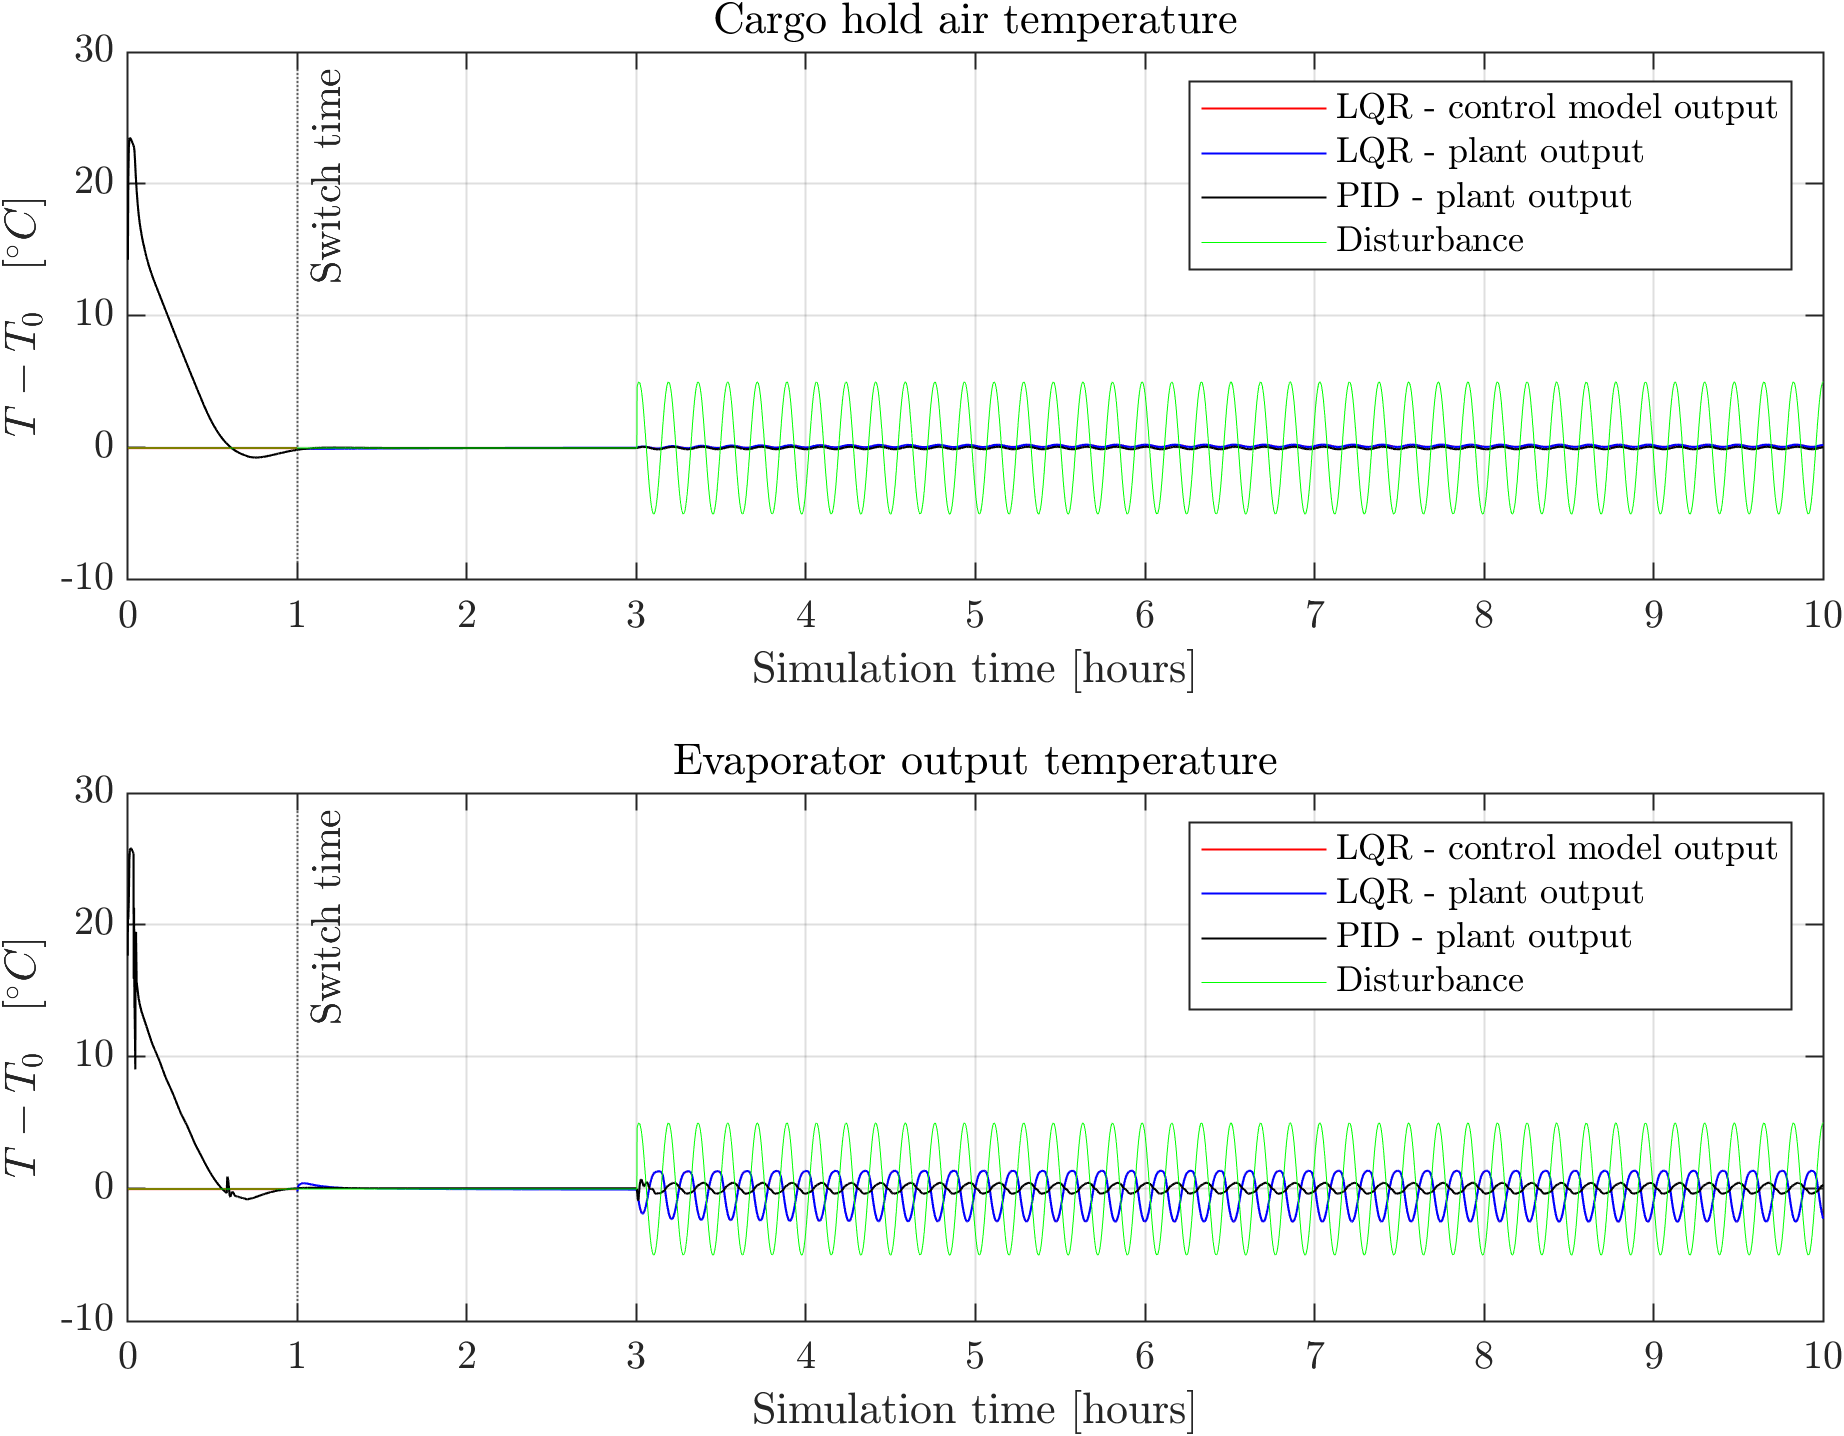
\includegraphics[width=0.8\textwidth]{Graphics/fig_LQRvsKresten_sineDist.png}
	\caption{Sine disturbance case: Top: Cargo hold air temperature. $T_0$ = -4.25$^{\circ}$C. Bottom: Evaporator vapor refridgerant temperature. $T_0$ = -5.55$^{\circ}$C}
	\label{fig:LQR_wellTuned_sineDist}
\end{figure}

\noindent \cref{fig:LQR_wellTuned_sineDist_zoom} shows a zoomed in version of \cref{fig:LQR_wellTuned_sineDist}, where the steady state behavior of the two outputs is seen.

\begin{figure}[H]
	\centering
	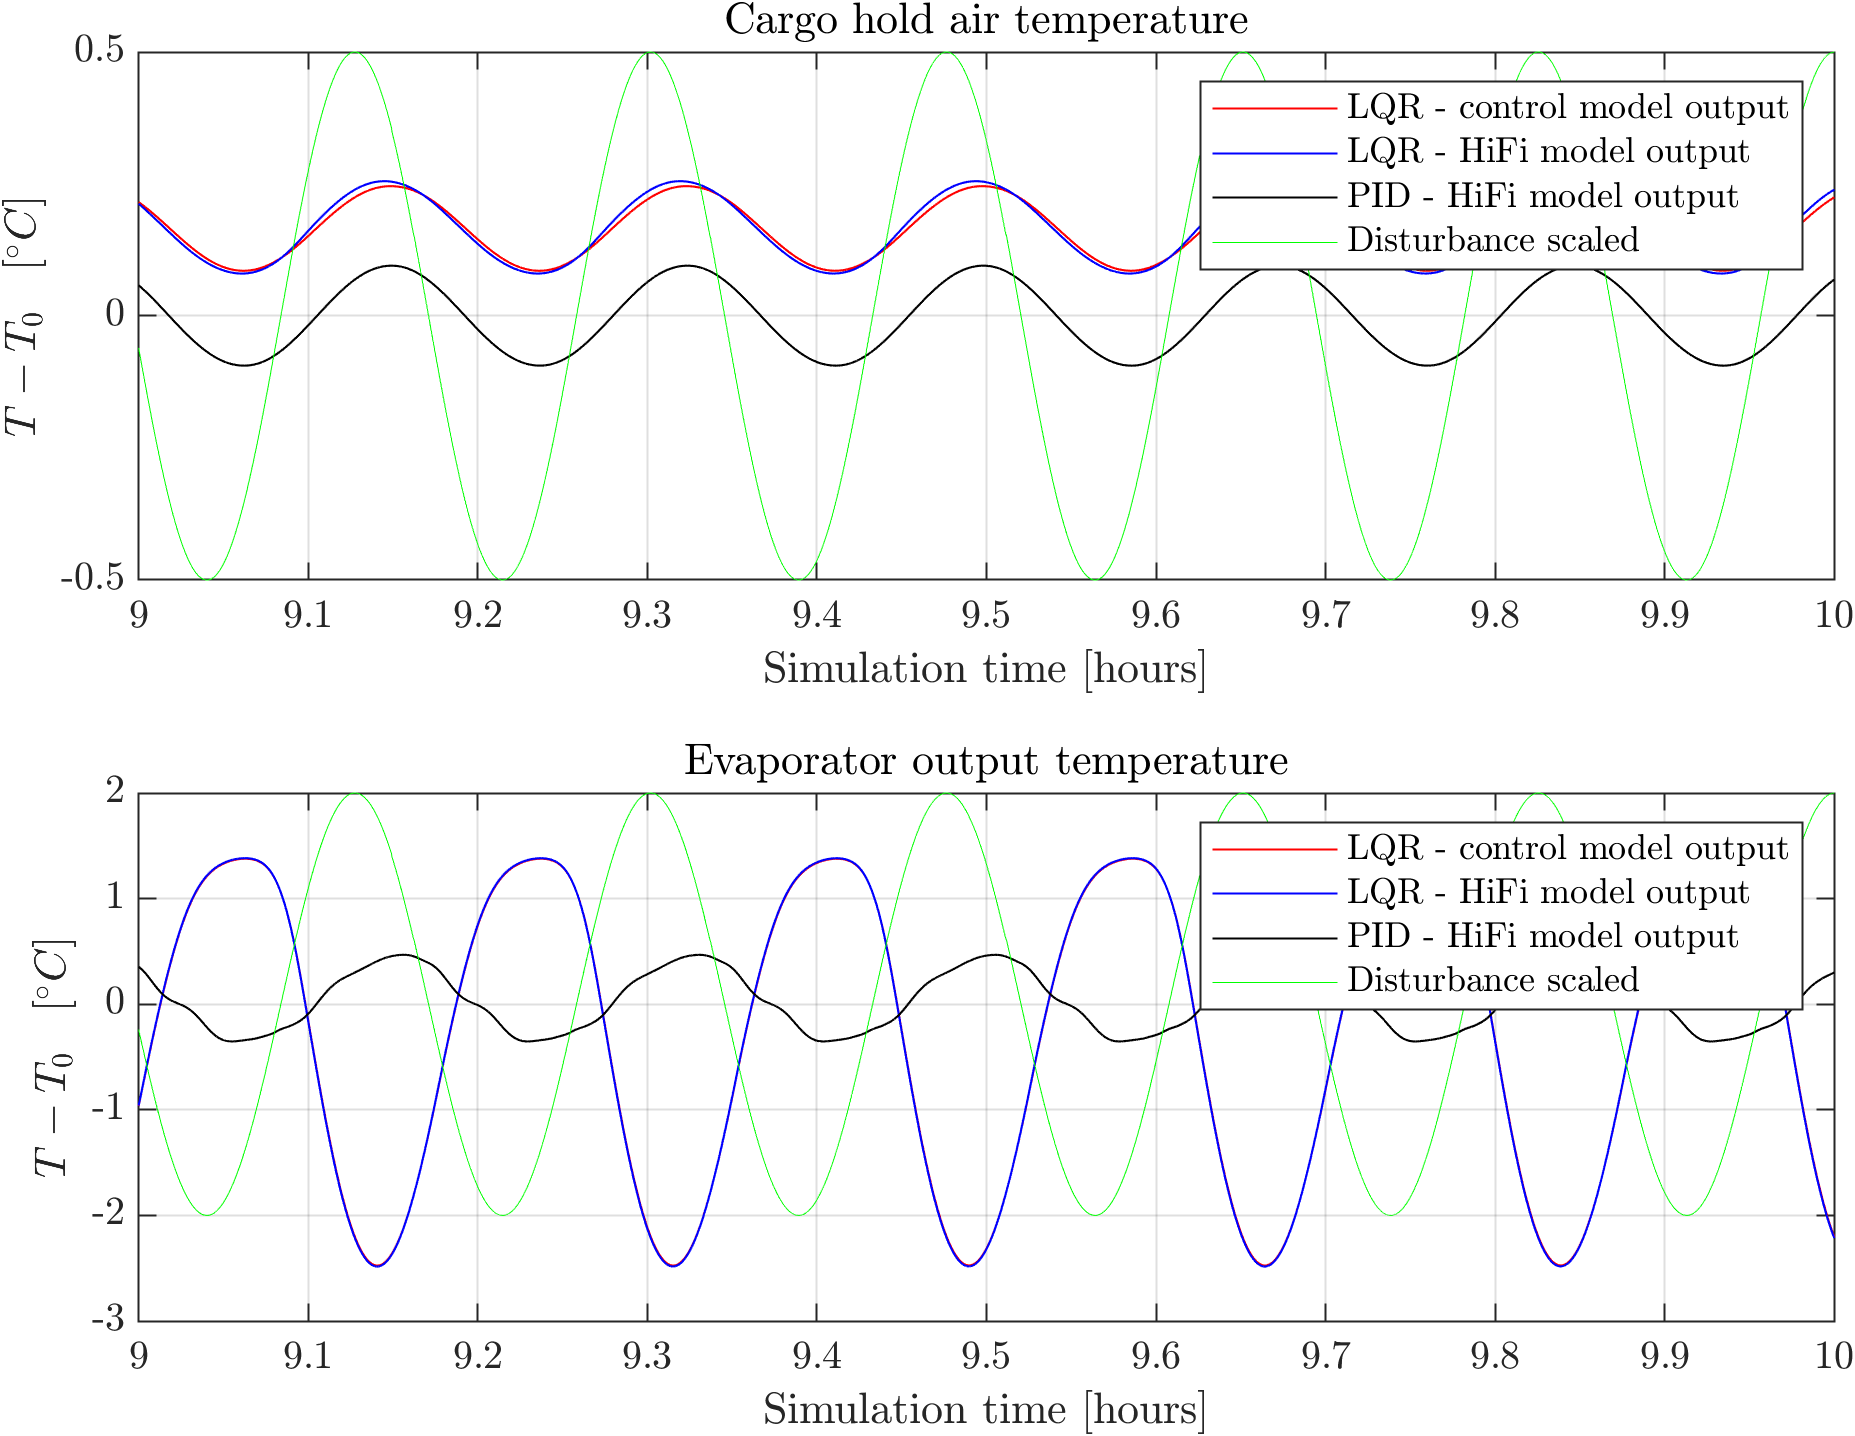
\includegraphics[width=0.8\textwidth]{Graphics/fig_LQRvsKresten_sineDist_zoom.png}
	\caption{Sine disturbance case: Top: Cargo hold air temperature. $T_0$ = -4.25$^{\circ}$C. Bottom: Evaporator vapor refrigerant temperature. $T_0$ = -5.55$^{\circ}$C}
	\label{fig:LQR_wellTuned_sineDist_zoom}
\end{figure}

\noindent A few interesting things are revealed in these plots. Firstly, the amplitude of the oscillations of $T_v$ are considerably lower with the PID control structure, than with the LQR controller. This implies that the optimal control strategy is less efficient in correcting errors on that particular state. Intuitively this would be improved by penalizing the relevant entry in the $Q$ weighing matrix. This has been attempted, and it was found that increasing the weight led to larger oscillations in the state.\\

It is likely that the main cause of this phenomenon, is the control model itself. Due to the simplifications made, and the Kalman decomposition, information about the unused inputs' ($\omega$, $U_{fan_1}$ and $\theta_2$) effect on the states was lost. It is expected that a controller (such as the PID structure), that is able to regulate these inputs would perform better, i.e. minimize the oscillations. This is further confirmed when looking at the inputs from the two different control structures in \cref{fig:inputs_sineDist} and \cref{fig:inputs_sineDist_zoom}. As expected the PID control structure utilizes all control inputs to minimize the disturbances effect on the system.\\

The oscillations on the cargo hold air temperature are not visibly different for the two control strategies. The amplitude of the oscillation is 0.18$^{\circ}$C. Thus the control strategy is performing well at minimizing an oscillating ambient temperatures effect on the air temperature inside the trailer.

\begin{figure}[H]
	\centering
	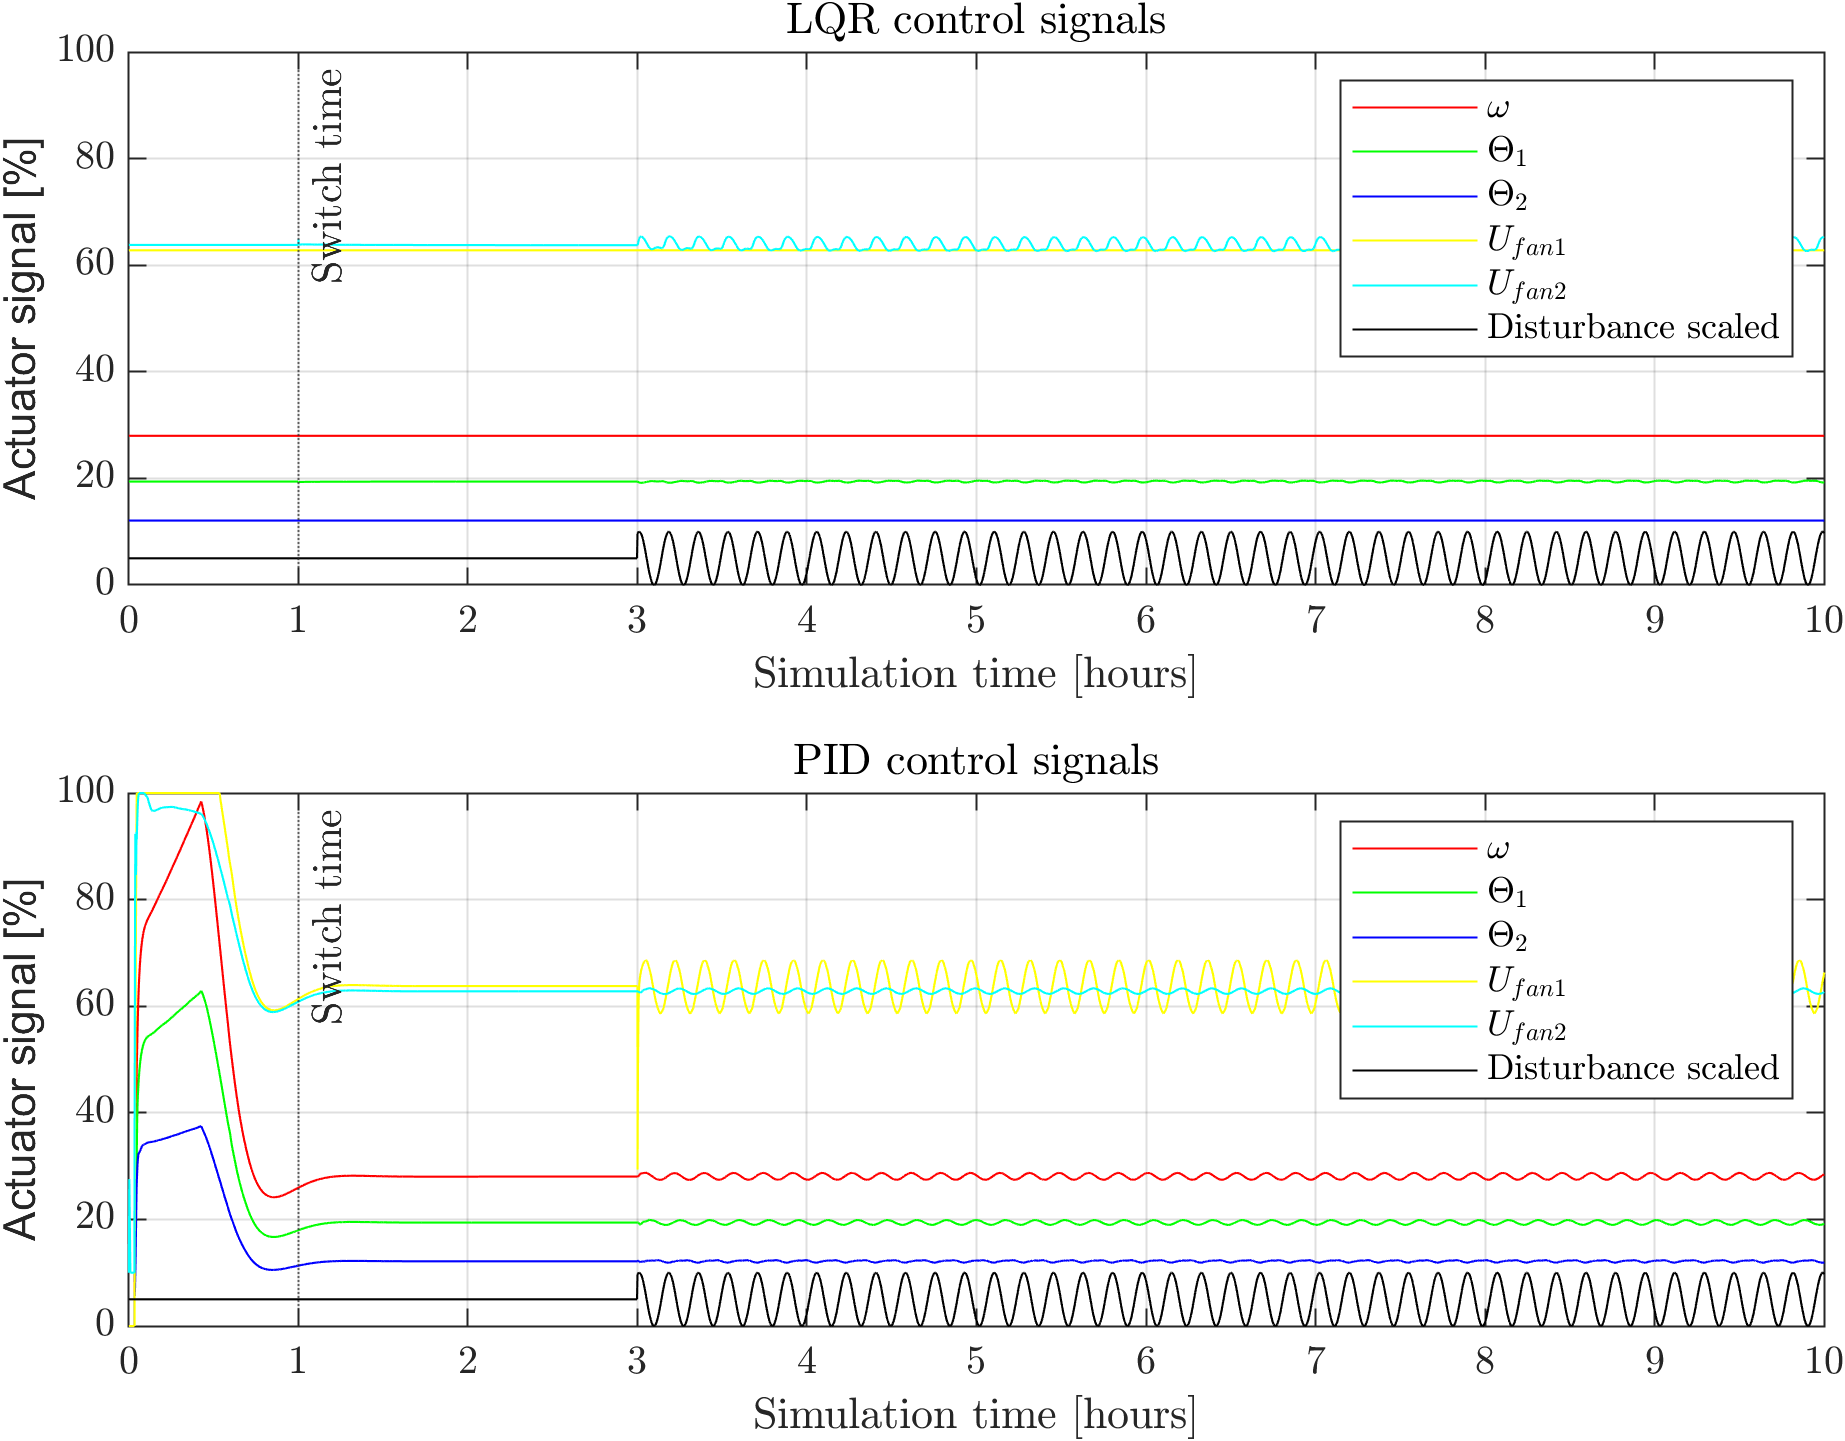
\includegraphics[width=0.8\textwidth]{Graphics/fig_inputs_sineDist.png}
	\caption{Sine disturbance case: Plot of the control signals applied to the Hi-Fi Simulation. Top: LQR control signals. Bottom: Hi-Fi simulation PID control signals.}
	\label{fig:inputs_sineDist}
\end{figure}

\begin{figure}[H]
	\centering
	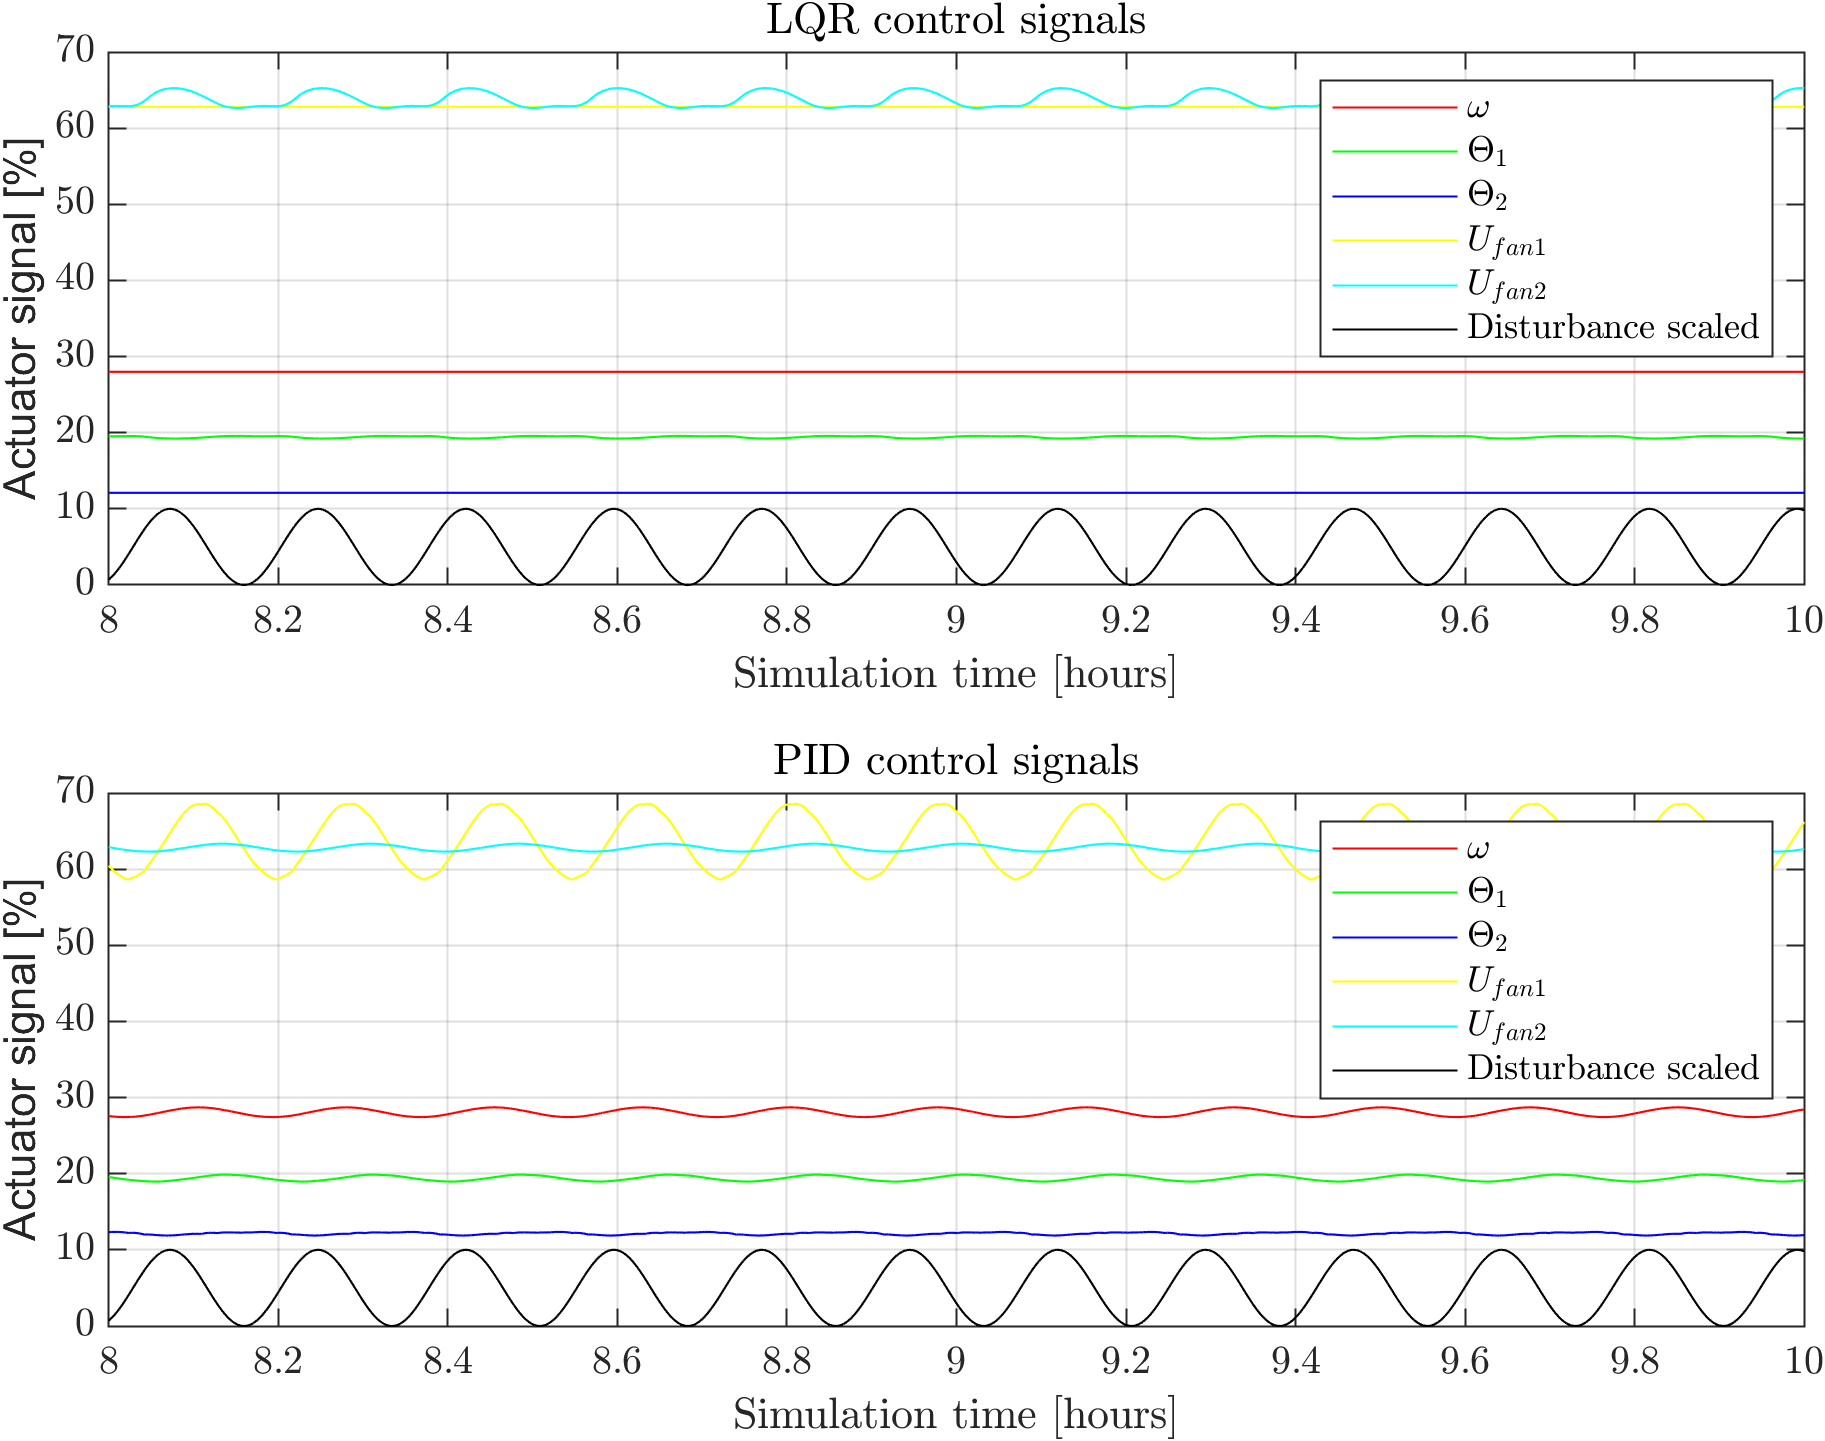
\includegraphics[width=0.8\textwidth]{Graphics/fig_inputs_sineDist_zoom.png}
	\caption{Sine disturbance case: Plot of the control signals applied to the Hi-Fi Simulation (zoomed). Top: LQR control signals. Bottom: Hi-Fi simulation PID control signals.}
	\label{fig:inputs_sineDist_zoom}
\end{figure}

\todo[inline]{Mention power consumption}

OBLQR: 25.32 kWh
PID: 25.21 kWh

\newpage
\subsection{Tuned LQR controller: Step disturbance}
To test the models ability to continuously perform outside the operating point, a step disturbance is applied to the ambient temperature.  At time $t=3$ hours, a 5$^{\circ}$C step in the disturbance is introduced. As before the PID structure handles the first hour of simulation, after which the optimal controller takes action. The controlled outputs are seen in \cref{fig:LQR_wellTuned_5stepDist}.

\begin{figure}[H]
	\centering
	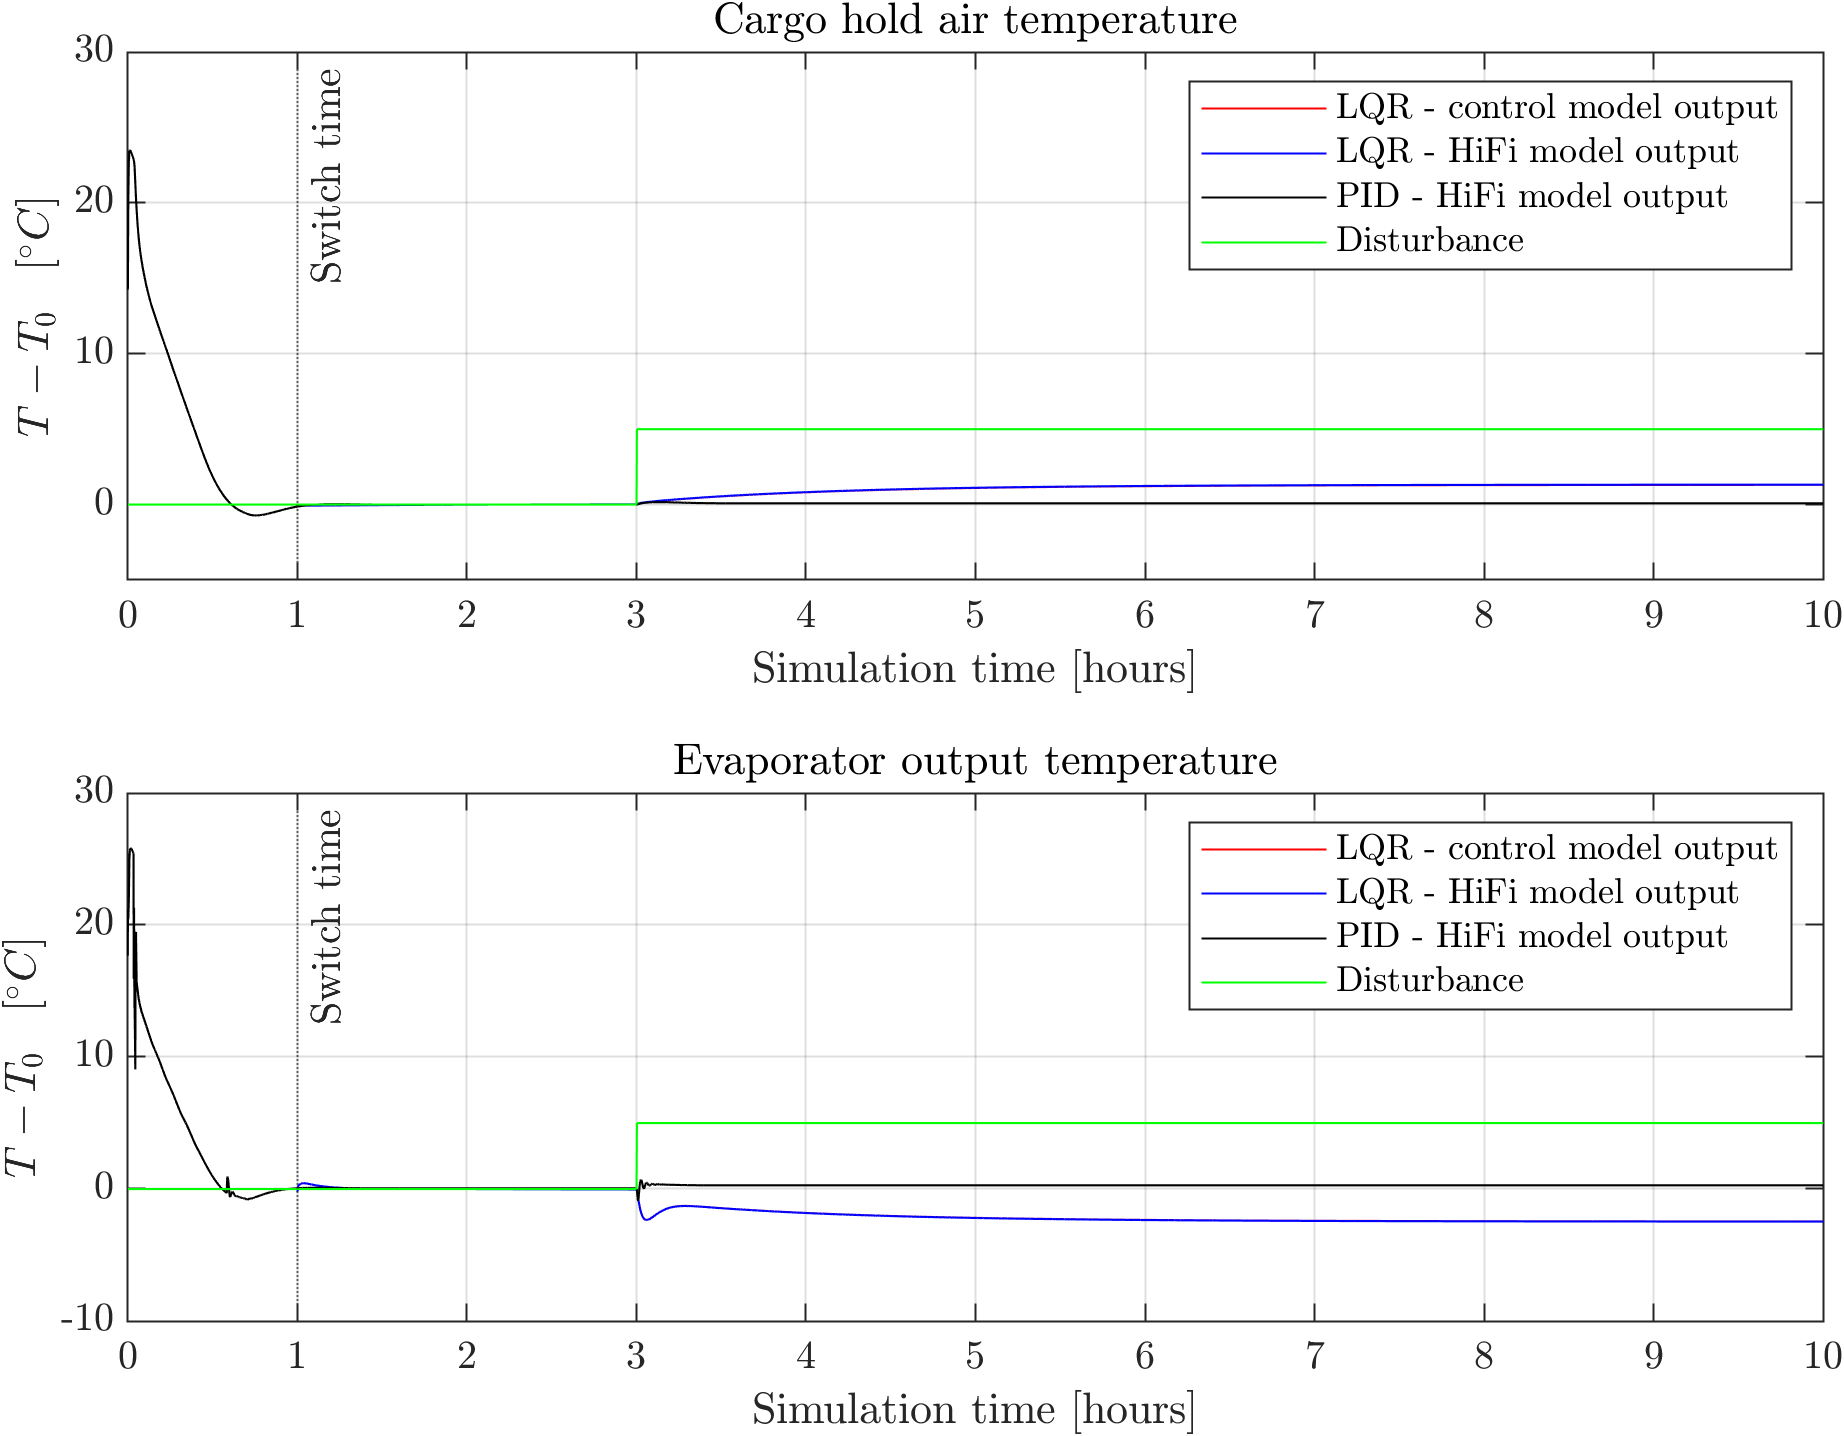
\includegraphics[width=0.8\textwidth]{Graphics/fig_LQRvsKresten_stepDist.png}
	\caption{Step disturbance case: Top: Cargo hold air temperature. $T_0$ = -4.25$^{\circ}$C. Bottom: Evaporator vapor refridgerant temperature. $T_0$ = -5.55$^{\circ}$C}
	\label{fig:LQR_wellTuned_5stepDist}
\end{figure}

\noindent \cref{fig:LQR_wellTuned_5stepDist_zoom} shows a zoomed in version of \cref{fig:LQR_wellTuned_5stepDist}, where the steady state error of the two outputs is seen.

\begin{figure}[H]
	\centering
	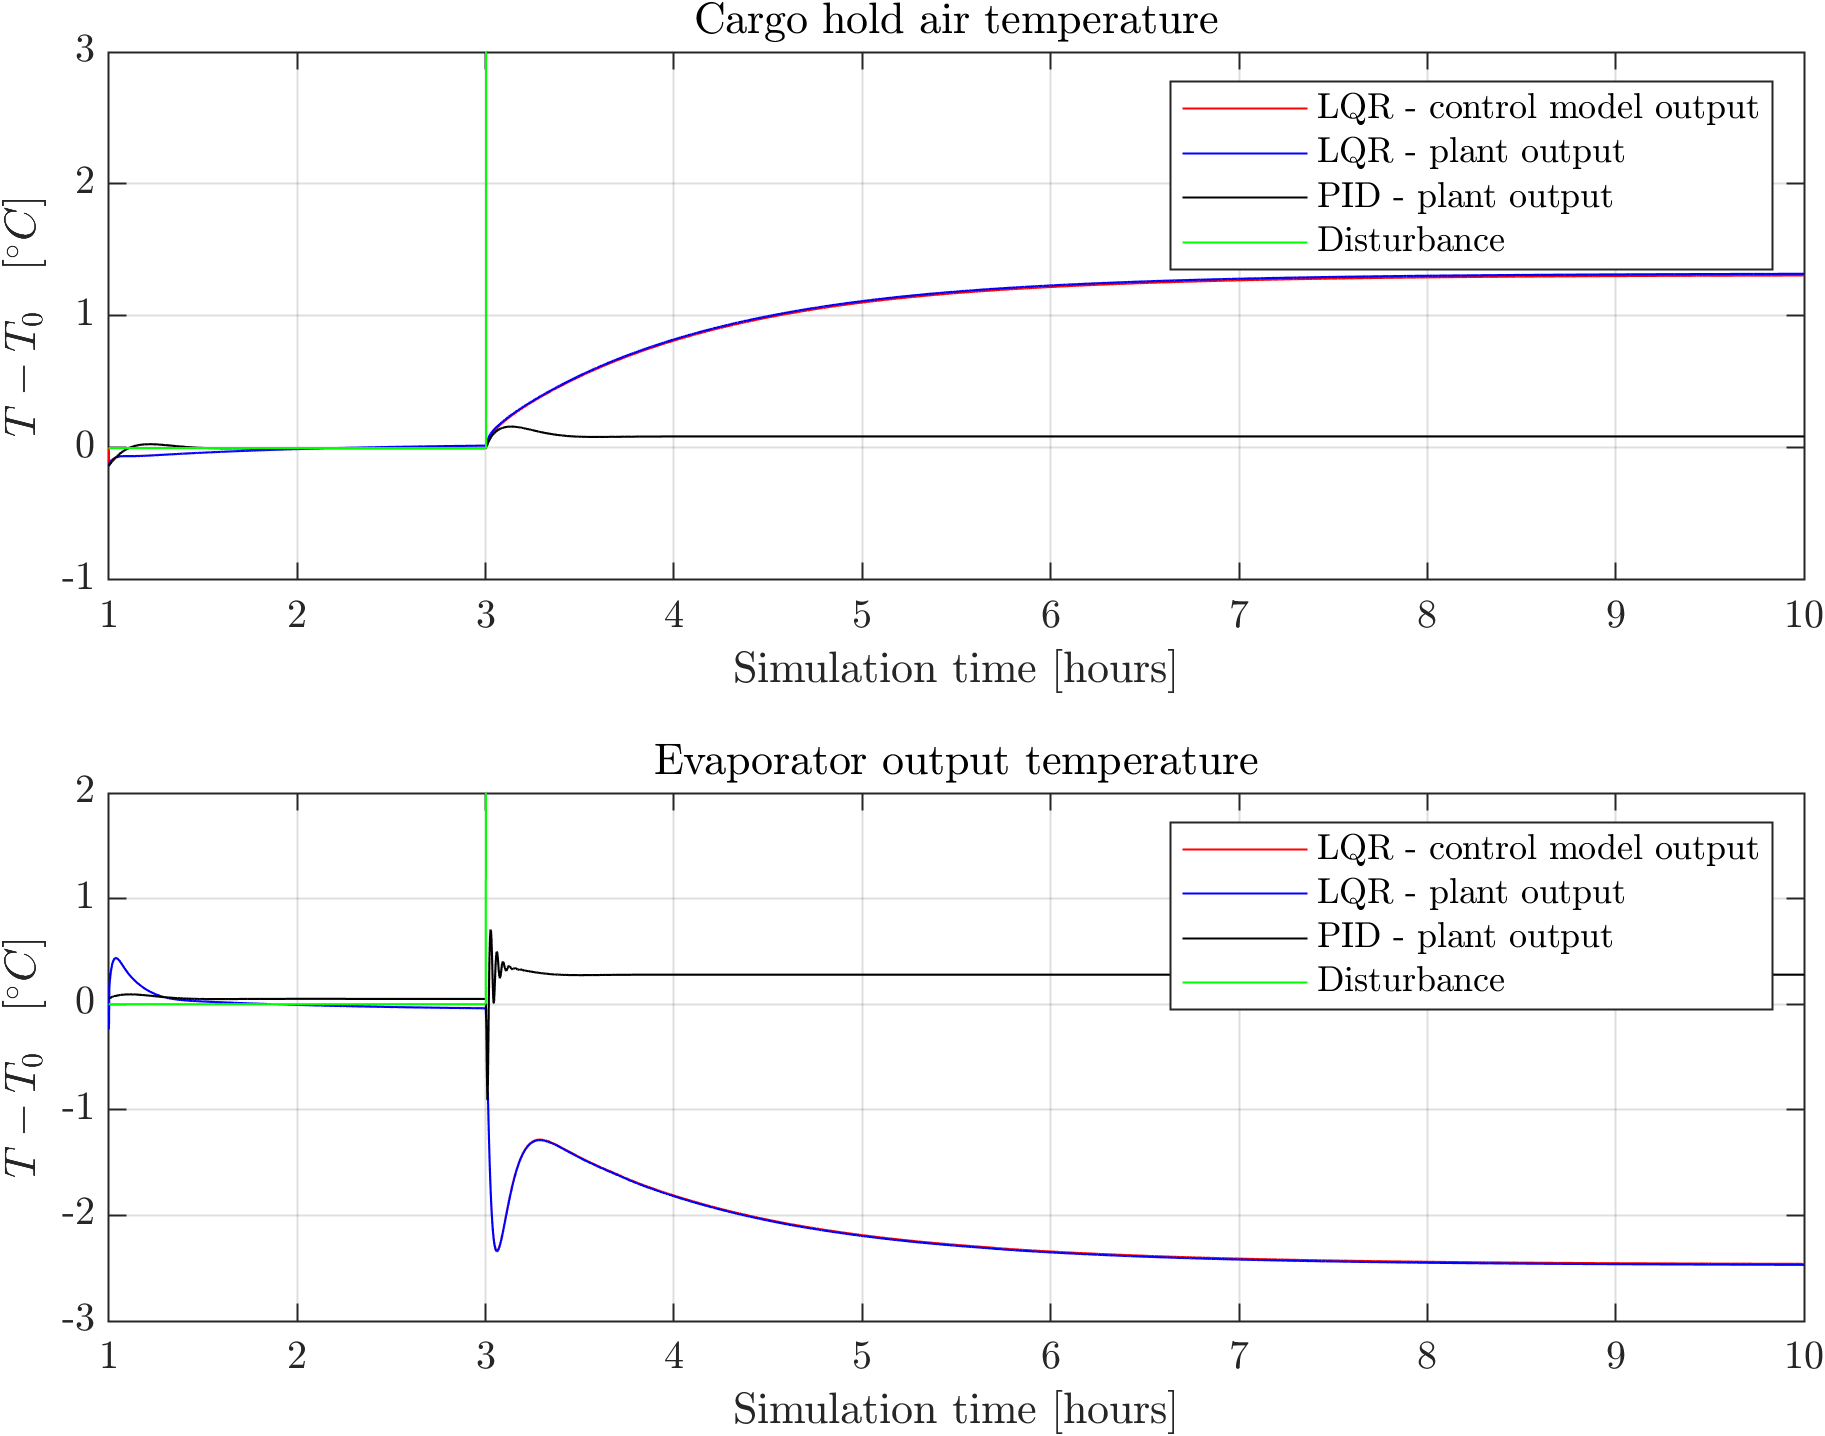
\includegraphics[width=0.8\textwidth]{Graphics/fig_LQRvsKresten_stepDist_zoom.png}
	\caption{Step disturbance case: Top: Cargo hold air temperature. $T_0$ = -4.25$^{\circ}$C. Bottom: Evaporator vapor refrigerant temperature. $T_0$ = -5.55$^{\circ}$C}
	\label{fig:LQR_wellTuned_5stepDist_zoom}
\end{figure}

\noindent It is seen that air temperature converges to 1.25$^{\circ}$C above the operating point, which means $T_{air} = -3^{\circ}C$. The superheat drops to 2.4$^{\circ}$C below the operating point, which means there is 3.6$^{\circ}$C superheat.\\

The increase in air temperature is large enough to be considered a problem for transportation of temperature critical goods, which is of course the intended purpose of the reefer trailer. The cause is likely, as was the case for the sine disturbance, that the controller is unable to change the compressor speed. The compressor speed is critical for increasing the refrigerant flow through the cycle, and is thus highly correlated with the cooling capacity of the system. \\

The drop in superheat is not as critical a problem as the air temperature. Ideally the controller would be able to keep it at the operating point, and in that context it is not desirable behavior. Technically, a drop in superheat increases the evaporation efficiency, and as long as there is a positive superheat no liquid will flow into the compressor. In summary, while the drop in superheat might increase efficiency without damaging the compressor, it would be a far more appealing if the controller was able to maintain the superheat at a fixed value.

The control inputs during this test is seen in \cref{fig:inputs_stepDist}.

\begin{figure}[H]
	\centering
	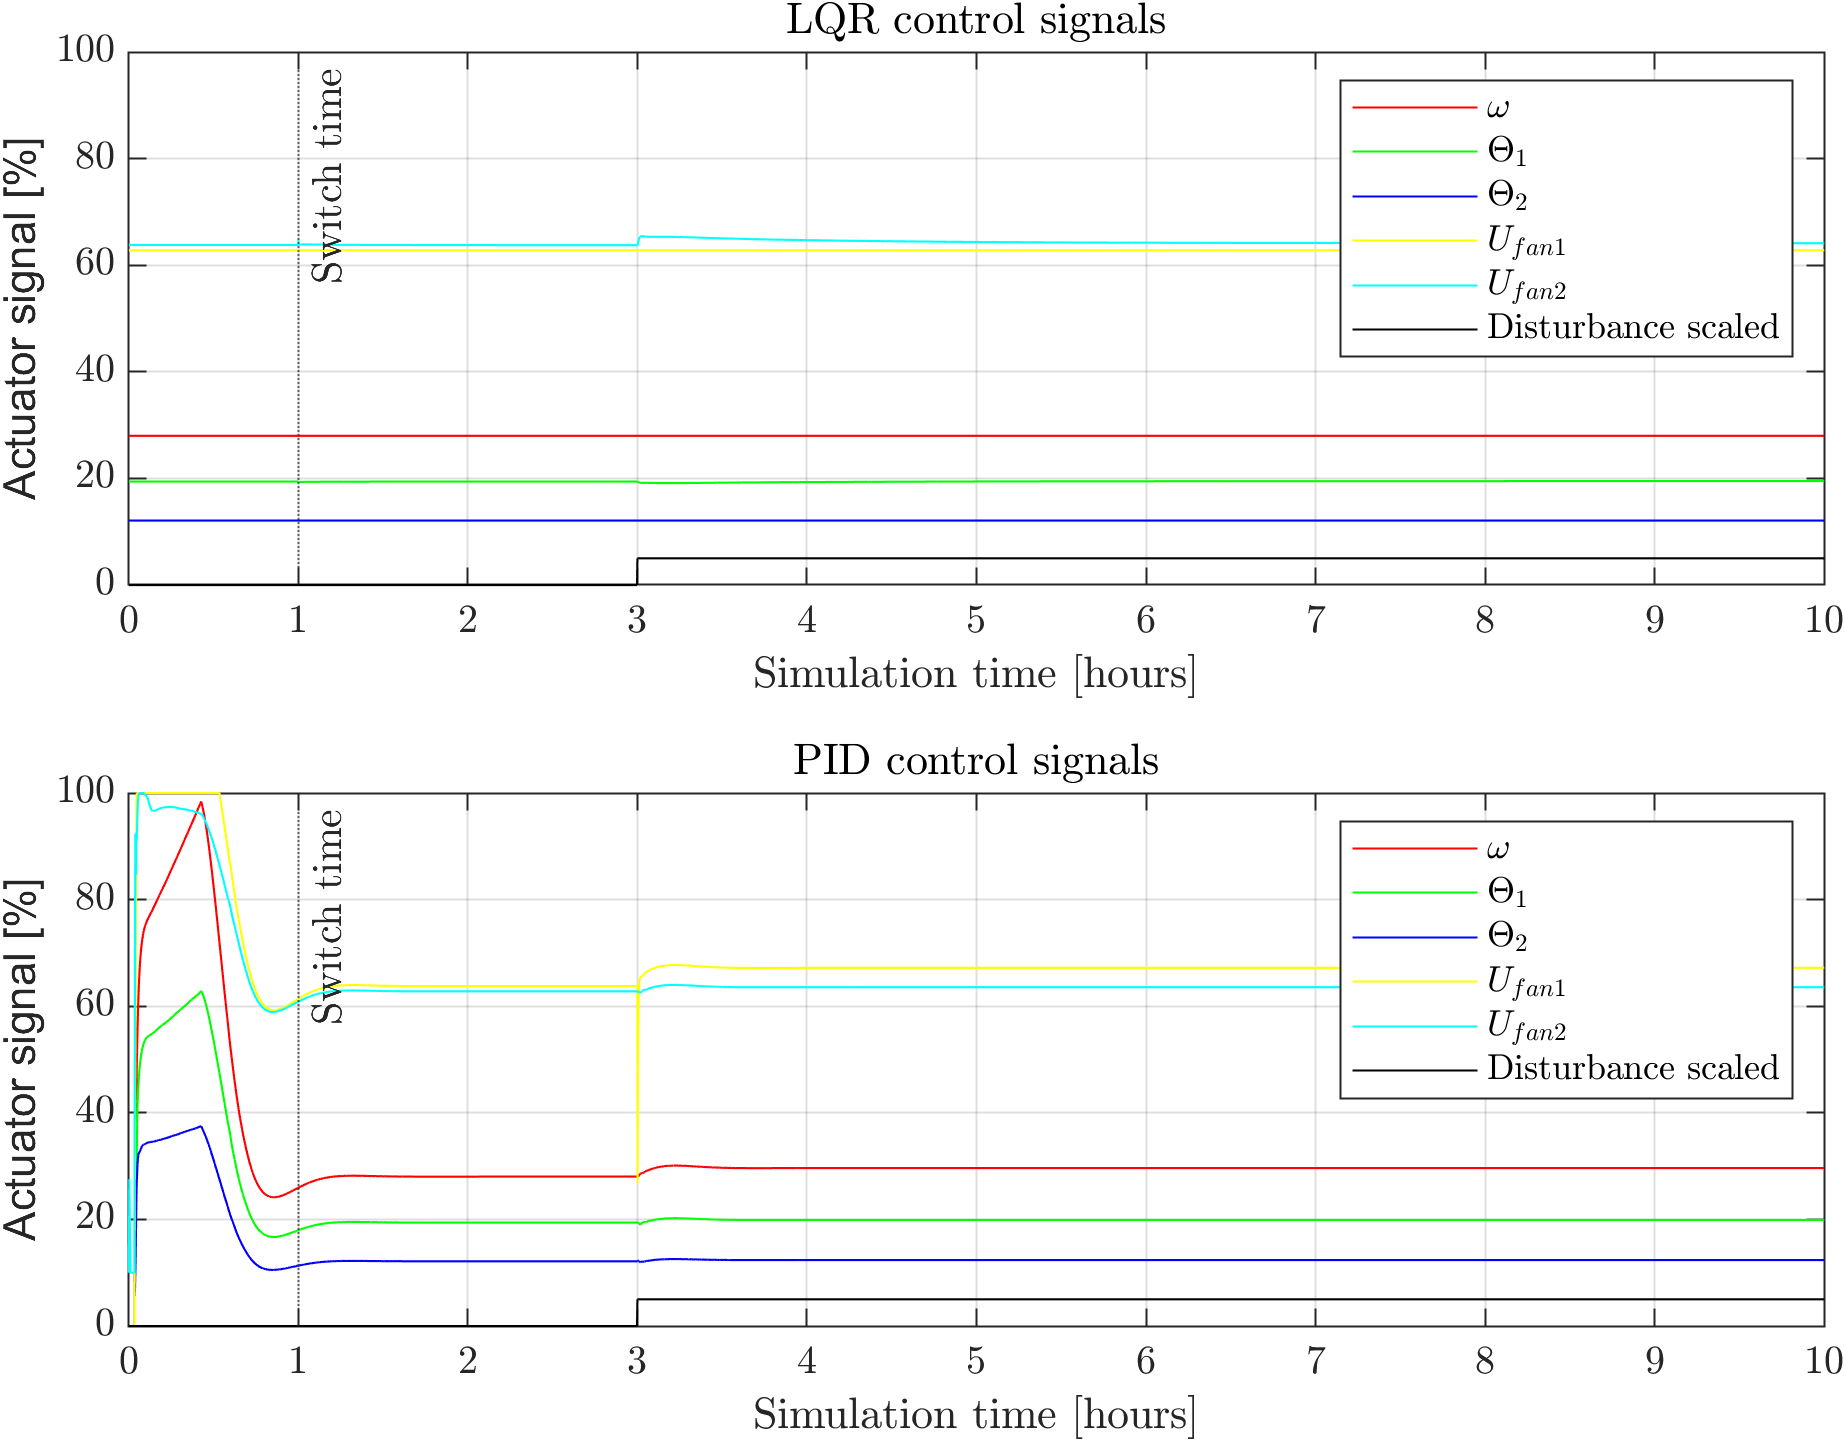
\includegraphics[width=0.8\textwidth]{Graphics/fig_inputs_stepDist.png}
	\caption{Step disturbance case: Plot of the control signals applied to the Hi-Fi Simulation. Top: LQR control signals. Bottom: Hi-Fi simulation PID control signals.}
	\label{fig:inputs_stepDist}
\end{figure}

\begin{figure}[H]
	\centering
	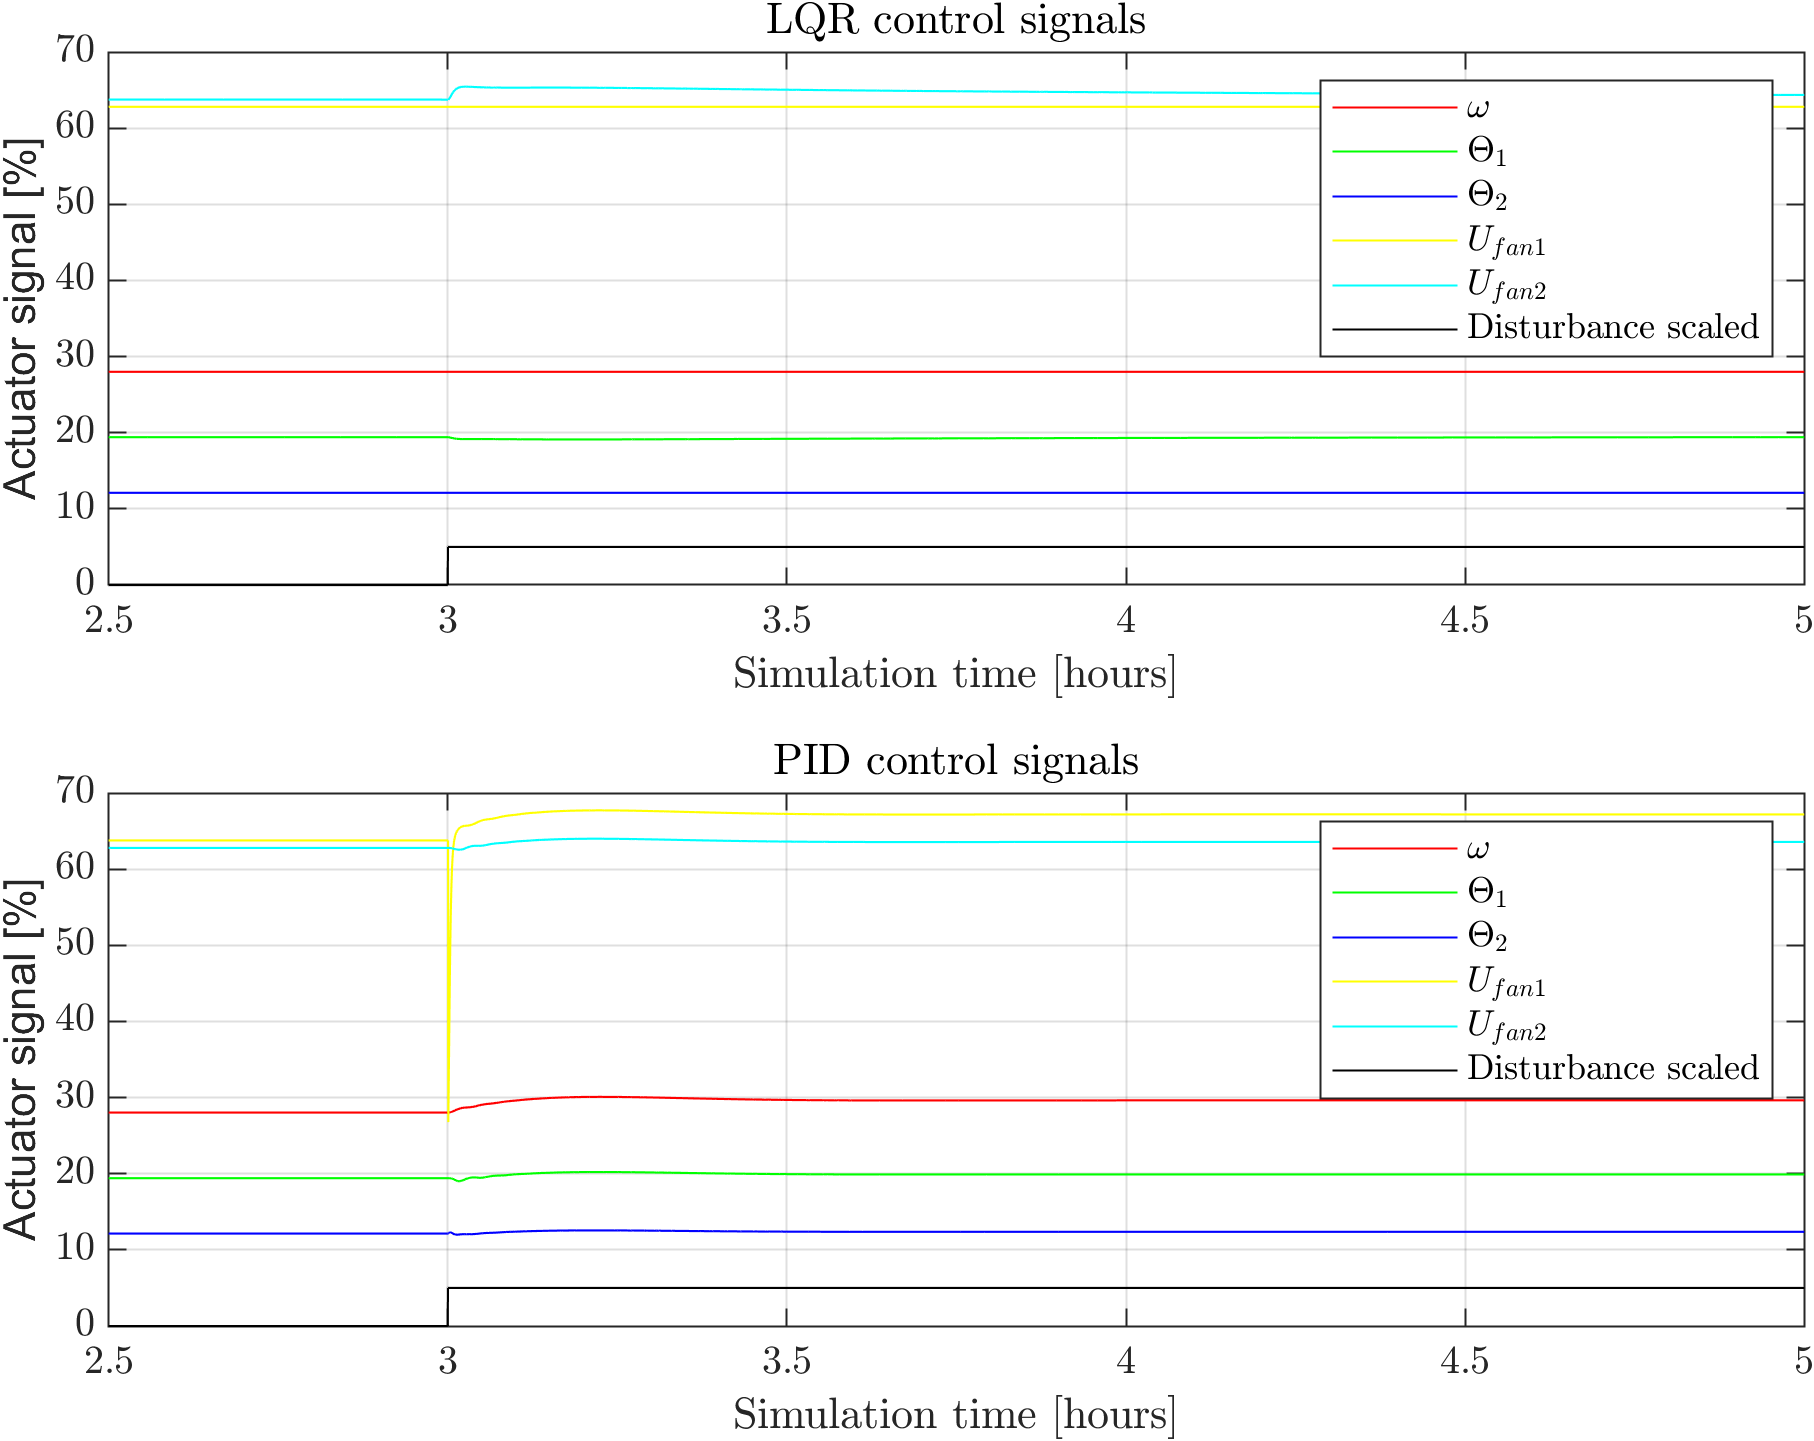
\includegraphics[width=0.8\textwidth]{Graphics/fig_inputs_stepDist_zoom.png}
	\caption{Step disturbance case: Plot of the control signals applied to the Hi-Fi Simulation (zoomed). Top: LQR control signals. Bottom: Hi-Fi simulation PID control signals.}
	\label{fig:inputs_stepDist_zoom}
\end{figure}

\todo[inline]{Mention power consumption}

OBLQR: 28.99 kWh
PID: 29.46 kWh

\subsubsection{conclude on the results.. }